\cleardoublepage\chapter{Performance analysis}\chaptermark{Performance analysis}\label{chap:performance}
\section{Sensor placement}
\subsection{Translation}
The general rule about sensor placement is that the closer the sensors are to each other, the more accurate the placing has to be. For example at the desired inter-sensor distance 2~m, a misplacement of 5~cm yields a 2.5~\% error in velocity. At the desired inter-sensor distance 0.2~m, a misplacement of 5~mm yields the same error. Since it is complex to sample too often, and by only considering sensor placement, the nodes in a sensor pair should be placed as far from each other as possible.

\subsection{Rotation}

When placing the sensor it is important that the axes point in the correct directions. However it is easy to accidentally rotate the sensor. The effect of rotating the sensor in the yaw ($\hat{z}$) and pitch ($\hat{y}$) axes can be seen in \mbox{Figures \ref{fig:xrotate} and \ref{fig:zrotate}.} If the rotation is known the software could easily correct for this.

\begin{subfigures}
\begin{figure}
 \centering
 \begin{minipage}{0.45\linewidth}
 \centering
  % generated by laprint.m
% %
% \begin{psfrags}%
% \psfragscanon%
%
% text strings:
\psfrag{s05}[b][b]{\fontsize{8}{12}\fontseries{m}\mathversion{normal}\fontshape{n}\selectfont \setlength{\tabcolsep}{0pt}\begin{tabular}{c}Magnetic field strength [nT]\end{tabular}}%
\psfrag{s06}[t][t]{\fontsize{8}{12}\fontseries{m}\mathversion{normal}\fontshape{n}\selectfont \setlength{\tabcolsep}{0pt}\begin{tabular}{c}Time [s]\end{tabular}}%
\psfrag{s07}[b][b]{\fontsize{8}{12}\fontseries{m}\mathversion{normal}\fontshape{n}\selectfont \setlength{\tabcolsep}{0pt}\begin{tabular}{c}Magnetic field strength for different sensor yaw angle.\end{tabular}}%
\psfrag{s10}[][]{\fontsize{10}{15}\fontseries{m}\mathversion{normal}\fontshape{n}\selectfont \setlength{\tabcolsep}{0pt}\begin{tabular}{c} \end{tabular}}%
\psfrag{s11}[][]{\fontsize{10}{15}\fontseries{m}\mathversion{normal}\fontshape{n}\selectfont \setlength{\tabcolsep}{0pt}\begin{tabular}{c} \end{tabular}}%
\psfrag{s12}[l][l]{\fontsize{6}{12}\fontseries{m}\mathversion{normal}\fontshape{n}\selectfont $\alpha = 90^\circ$}%
\psfrag{s13}[l][l]{\fontsize{6}{12}\fontseries{m}\mathversion{normal}\fontshape{n}\selectfont $\alpha = 0^\circ$}%
\psfrag{s14}[l][l]{\fontsize{6}{12}\fontseries{m}\mathversion{normal}\fontshape{n}\selectfont $\alpha = 30^\circ$}%
\psfrag{s15}[l][l]{\fontsize{6}{12}\fontseries{m}\mathversion{normal}\fontshape{n}\selectfont $\alpha = 60^\circ$}%
\psfrag{s16}[l][l]{\fontsize{6}{12}\fontseries{m}\mathversion{normal}\fontshape{n}\selectfont $\alpha = 90^\circ$}%
%
% axes font properties:
\fontsize{6}{12}\fontseries{m}\mathversion{normal}%
\fontshape{n}\selectfont%
%
% xticklabels:
\psfrag{x01}[t][t]{-0.5}%
\psfrag{x02}[t][t]{0}%
\psfrag{x03}[t][t]{0.5}%
%
% yticklabels:
\psfrag{v01}[r][r]{-60}%
\psfrag{v02}[r][r]{-40}%
\psfrag{v03}[r][r]{-20}%
\psfrag{v04}[r][r]{0}%
\psfrag{v05}[r][r]{20}%
\psfrag{v06}[r][r]{40}%
%
% Figure:
% \resizebox{6cm}{!}{\includegraphics{xrotate.eps}}%
% \end{psfrags}%
%
% End xrotate.tex

  \includegraphics[width=1\linewidth]{images/xrotate}
 % sensoraxis.eps: 1179666x1179666 pixel, 300dpi, 9987.84x9987.84 cm, bb=
 \caption[Effect of sensor node rotation. Yaw axis.]{Effect of sensor node rotation. The sensor is rotated around its yaw axis and the effect on the $\hat{\vec{x}}$-axis can be seen.}
 \label{fig:xrotate}
 \end{minipage}\hfill
 \begin{minipage}{0.45\linewidth}
 \centering
 % % generated by laprint.m
% %
% \begin{psfrags}%
% \psfragscanon%
%
% text strings:
\psfrag{s05}[b][b]{\fontsize{8}{12}\fontseries{m}\mathversion{normal}\fontshape{n}\selectfont \setlength{\tabcolsep}{0pt}\begin{tabular}{c}Magnetic field strength [nT]\end{tabular}}%
\psfrag{s06}[t][t]{\fontsize{8}{12}\fontseries{m}\mathversion{normal}\fontshape{n}\selectfont \setlength{\tabcolsep}{0pt}\begin{tabular}{c}Time [s]\end{tabular}}%
\psfrag{s07}[b][b]{\fontsize{8}{12}\fontseries{m}\mathversion{normal}\fontshape{n}\selectfont \setlength{\tabcolsep}{0pt}\begin{tabular}{c}Magnetic field strength for different sensor pitch angle.\end{tabular}}%
\psfrag{s10}[][]{\fontsize{10}{15}\fontseries{m}\mathversion{normal}\fontshape{n}\selectfont \setlength{\tabcolsep}{0pt}\begin{tabular}{c} \end{tabular}}%
\psfrag{s11}[][]{\fontsize{10}{15}\fontseries{m}\mathversion{normal}\fontshape{n}\selectfont \setlength{\tabcolsep}{0pt}\begin{tabular}{c} \end{tabular}}%
\psfrag{s12}[l][l]{\fontsize{6}{15}\fontseries{m}\mathversion{normal}\fontshape{n}\selectfont $\beta = 90^\circ$}%
\psfrag{s13}[l][l]{\fontsize{6}{15}\fontseries{m}\mathversion{normal}\fontshape{n}\selectfont $\beta = 0^\circ$}%
\psfrag{s14}[l][l]{\fontsize{6}{15}\fontseries{m}\mathversion{normal}\fontshape{n}\selectfont $\beta = 30^\circ$}%
\psfrag{s15}[l][l]{\fontsize{6}{15}\fontseries{m}\mathversion{normal}\fontshape{n}\selectfont $\beta = 60^\circ$}%
\psfrag{s16}[l][l]{\fontsize{6}{15}\fontseries{m}\mathversion{normal}\fontshape{n}\selectfont $\beta = 90^\circ$}%
%
% axes font properties:
\fontsize{6}{15}\fontseries{m}\mathversion{normal}%
\fontshape{n}\selectfont%
%
% xticklabels:
\psfrag{x01}[t][t]{-0.5}%
\psfrag{x02}[t][t]{0}%
\psfrag{x03}[t][t]{0.5}%
%
% yticklabels:
\psfrag{v01}[r][r]{-100}%
\psfrag{v02}[r][r]{-50}%
\psfrag{v03}[r][r]{0}%
\psfrag{v04}[r][r]{50}%
\psfrag{v05}[r][r]{100}%
%
% % Figure:
% \resizebox{6cm}{!}{\includegraphics{zrotate.eps}}%
% \end{psfrags}%
% %
% End zrotate.tex

  \includegraphics[width=1\linewidth]{images/zrotate}
 % sensoraxis.eps: 1179666x1179666 pixel, 300dpi, 9987.84x9987.84 cm, bb=
 \caption[Effect of sensor node rotation. Pitch axis.]{Effect of sensor node rotation. The sensor is rotated around its pitch axis and the effect on the $\hat{\vec{z}}$-axis can be seen.}
 \label{fig:zrotate}
 \end{minipage}
\end{figure}
\end{subfigures}

\section{Detection}\index{direction}
In the simulator a number of potential problems have been identified. If two vehicles are travelling close to each other, especially if they are large, the signal will be indistinguishable from a single very long vehicle. This can be combated by placing the sensor as close to the vehicles as possible.  Similarly, a vehicle in an adjacent lane will disturb our signal. This is remedied by choosing the threshold value wisely. Some vehicles such as motorcycles and some small cars will not produce a signal with high enough magnitude. Placing the sensor closer to the vehicle will help, more sensors will ensure that the vehicle pass at least one sensor.

In the real-life tests performed, we detected 100~\% of normal-sized vehicles. The vehicles not detected were bicycles and a very small motorcycle. The signature from each vehicle was clearly visible, and could be both seen by eye or by a simple counting algorithm. The simulations displayed very similar vehicle signatures, but not all vehicles were detected due to the minimum distance between vehicles set in the simulator. In the real life test there were no vehicles travelling bumper to bumper which was expected due to the comparably high speed.

\section{Speed estimation}\index{speed estimation}

\subsection{Speed of an individual vehicle}
\subsubsection{Traditional time difference}
\begin{align}
 v_{\text{est}} &= \frac{d\left(t_{2,\text{on}}-t_{1,\text{on}}+ t_{2,\text{off}} - t_{1,\text{off}}\right)}{(t_{2,\text{on}}-t_{1,\text{on}})(t_{2,\text{off}} - t_{1,\text{off}})+ \varepsilon\left([t_{2,\text{on}}-t_{1,\text{on}}]- [t_{2,\text{off}} - t_{1,\text{off}}]\right) + \varepsilon^2}.
  \label{eq:speed2}
\end{align}
The term $\varepsilon\left([t_{2,\text{on}}-t_{1,\text{on}}]- [t_{2,\text{off}} - t_{1,\text{off}}]\right)$ in \eqref{eq:speed2} is small if the signature is equal or similar at both sensors. In contrast to the conclusion in~\cite{path2007}, the term $\varepsilon^2$ is small, but not zero. If we assume a sampling speed of 100~Hz, a velocity of 72~km/h, a sensor separation of 2~m and $\varepsilon = 2$~samples then the sensitivity\index{sensitivity} parameter $\varepsilon^2$ introduces an error of 4~\%. If the distance is doubled, the error is 1~\%. The speed is a factor, a higher speed means less accuracy -- see Figure~\ref{fig:vest_eps}.

\begin{figure}[!thb]
  \centering
  \begin{minipage}{0.45\linewidth}
  \centering
  % % generated by laprint.m
% %
% \begin{psfrags}%
% \psfragscanon%
%
% text strings:
\psfrag{s05}[t][t]{\fontsize{8}{12}\fontseries{m}\mathversion{normal}\fontshape{n}\selectfont \setlength{\tabcolsep}{0pt}\begin{tabular}{c}$\varepsilon$ [s]\end{tabular}}%
\psfrag{s06}[b][b]{\fontsize{8}{12}\fontseries{m}\mathversion{normal}\fontshape{n}\selectfont \setlength{\tabcolsep}{0pt}\begin{tabular}{c}Error [\%]\end{tabular}}%
\psfrag{s07}[b][b]{\fontsize{8}{12}\fontseries{m}\mathversion{normal}\fontshape{n}\selectfont \setlength{\tabcolsep}{0pt}\begin{tabular}{c}Error due to sensitivity difference\end{tabular}}%
\psfrag{s10}[][]{\fontsize{8}{12}\fontseries{m}\mathversion{normal}\fontshape{n}\selectfont \setlength{\tabcolsep}{0pt}\begin{tabular}{c} \end{tabular}}%
\psfrag{s11}[][]{\fontsize{8}{12}\fontseries{m}\mathversion{normal}\fontshape{n}\selectfont \setlength{\tabcolsep}{0pt}\begin{tabular}{c} \end{tabular}}%
\psfrag{s12}[l][l]{\fontsize{6}{8}\fontseries{m}\mathversion{normal}\fontshape{n}\selectfont 110 km/h}%
\psfrag{s13}[l][l]{\fontsize{6}{8}\fontseries{m}\mathversion{normal}\fontshape{n}\selectfont 50 km/h}%
\psfrag{s14}[l][l]{\fontsize{6}{8}\fontseries{m}\mathversion{normal}\fontshape{n}\selectfont 70 km/h}%
\psfrag{s15}[l][l]{\fontsize{6}{8}\fontseries{m}\mathversion{normal}\fontshape{n}\selectfont 90 km/h}%
\psfrag{s16}[l][l]{\fontsize{6}{8}\fontseries{m}\mathversion{normal}\fontshape{n}\selectfont 110 km/h}%
%
% axes font properties:
\fontsize{8}{12}\fontseries{m}\mathversion{normal}%
\fontshape{n}\selectfont%
%
% xticklabels:
\psfrag{x01}[t][t]{$-0.02$}%
\psfrag{x02}[t][t]{$-0.01$}%
\psfrag{x03}[t][t]{$0$}%
\psfrag{x04}[t][t]{$0.01$}%
\psfrag{x05}[t][t]{$0.02$}%
%
% yticklabels:
\psfrag{v01}[r][r]{$0$}%
\psfrag{v02}[r][r]{$2$}%
\psfrag{v03}[r][r]{$4$}%
\psfrag{v04}[r][r]{$6$}%
\psfrag{v05}[r][r]{$8$}%
\psfrag{v06}[r][r]{$10$}%
\psfrag{v07}[r][r]{$12$}%
%
% Figure:
% \resizebox{6cm}{!}{\includegraphics{vest_eps.eps}}%
% \end{psfrags}%
%
% End vest_eps.tex

   \includegraphics[width=\linewidth]{images/vest_eps}
  \caption[Time difference. Error due to sensor sensitivity difference]{Time difference. Error due to sensor sensitivity difference. The distance between sensors was 2 m, and the speed was 20~m/s.}
  \label{fig:vest_eps}
  \end{minipage}
\end{figure}

\subsubsection[Comparison between traditional time difference and time difference using matched filter]{Comparison between traditional time\\difference and time difference using matched filter}

A comparison between the traditional and matched filter\index{matched filter} methods can be found in Figures \ref{fig:comp_mean_z}, \ref{fig:comp_std_z}, \ref{fig:comp_mean_y}, \ref{fig:comp_std_y}, \ref{fig:comp_mean_z_bus} and \ref{fig:comp_std_z_bus}. In Figures \ref{fig:comp_std_r} and \ref{fig:comp_std_r} we can see the result if we use the Euclidean norm $\Vert \vec{B} \Vert= \sqrt{B_x^2+B_y^2+B_z^2}$. We can see that the standard deviation of the matched filter\index{matched filter} (MF) method is much smaller than the standard deviation for the traditional method, or peak to peak (P-P) method regardless of SNR and sensor axis. We can see that the use of a lowpass filter\index{lowpass filter} (LP) on the first signal introduces an expected delay into the system. This filtering is done since we know we are not looking for an exact replica of the first signal and its noise, but rather a copy of the first clean signal with added, different, noise. This delay is of course known and can be compensated for. A lowpass filter will cause the time difference to be underestimated, and therefore the speed will be overestimated. We also note that it is beneficial to use the more complex $y$-axis.

For all of these simulations, the sensors were placed 1.5~m from the passing vehicle, and the SNR was varied between $\sim0{}$~dB and 40~dB. The vehicle speed was 72~km/h.

If we plot the mean error and error standard deviation versus the speed, we will see that the error and the error standard deviation goes to zero at higher speeds for the matched filter method. The result can be seen in \mbox{Figures \ref{fig:comp_mean-vel} and \ref{fig:comp_std-vel}.}

\begin{subfigures}
\begin{figure}[!tbh]
  \centering
  \begin{minipage}{0.45\linewidth}
  \centering
  % generated by laprint.m
%
% \begin{psfrags}%
% \psfragscanon%
%
% text strings:
\psfrag{s05}[b][b]{\fontsize{8}{12}\fontseries{m}\mathversion{normal}\fontshape{n}\selectfont \setlength{\tabcolsep}{0pt}\begin{tabular}{c}Comparison between time difference methods\end{tabular}}%
\psfrag{s06}[t][t]{\fontsize{8}{12}\fontseries{m}\mathversion{normal}\fontshape{n}\selectfont \setlength{\tabcolsep}{0pt}\begin{tabular}{c}SNR [dB]\end{tabular}}%
\psfrag{s07}[b][b]{\fontsize{8}{12}\fontseries{m}\mathversion{normal}\fontshape{n}\selectfont \setlength{\tabcolsep}{0pt}\begin{tabular}{c}Mean error [samples]\end{tabular}}%
\psfrag{s10}[][]{\fontsize{10}{15}\fontseries{m}\mathversion{normal}\fontshape{n}\selectfont \setlength{\tabcolsep}{0pt}\begin{tabular}{c} \end{tabular}}%
\psfrag{s11}[][]{\fontsize{4}{6}\fontseries{m}\mathversion{normal}\fontshape{n}\selectfont \setlength{\tabcolsep}{0pt}\begin{tabular}{c} \end{tabular}}%
\psfrag{s12}[l][l]{\fontsize{4}{6}\fontseries{m}\mathversion{normal}\fontshape{n}\selectfont MF LP}%
\psfrag{s13}[l][l]{\fontsize{4}{6}\fontseries{m}\mathversion{normal}\fontshape{n}\selectfont P-P}%
\psfrag{s14}[l][l]{\fontsize{4}{6}\fontseries{m}\mathversion{normal}\fontshape{n}\selectfont P-P LP}%
\psfrag{s15}[l][l]{\fontsize{4}{6}\fontseries{m}\mathversion{normal}\fontshape{n}\selectfont MF}%
\psfrag{s16}[l][l]{\fontsize{4}{6}\fontseries{m}\mathversion{normal}\fontshape{n}\selectfont MF LP}%
%
% axes font properties:
\fontsize{6}{8}\fontseries{m}\mathversion{normal}%
\fontshape{n}\selectfont%
%
% xticklabels:
\psfrag{x01}[t][t]{$0$}%
\psfrag{x02}[t][t]{$5$}%
\psfrag{x03}[t][t]{$10$}%
\psfrag{x04}[t][t]{$15$}%
\psfrag{x05}[t][t]{$20$}%
\psfrag{x06}[t][t]{$25$}%
\psfrag{x07}[t][t]{$30$}%
\psfrag{x08}[t][t]{$35$}%
\psfrag{x09}[t][t]{$40$}%
%
% yticklabels:
\psfrag{v01}[r][r]{$0$}%
\psfrag{v02}[r][r]{$0.1$}%
\psfrag{v03}[r][r]{$0.2$}%
\psfrag{v04}[r][r]{$0.3$}%
\psfrag{v05}[r][r]{$0.4$}%
\psfrag{v06}[r][r]{$0.5$}%
\psfrag{v07}[r][r]{$0.6$}%
\psfrag{v08}[r][r]{$0.7$}%
\psfrag{v09}[r][r]{$0.8$}%
\psfrag{v10}[r][r]{$0.9$}%
\psfrag{v11}[r][r]{$1$}%
%
% Figure:
% \resizebox{6cm}{!}{\includegraphics{mean_error_z.eps}}%
% \end{psfrags}%
%
% End mean_error_z.tex

   \includegraphics[width=\linewidth]{images/mean_error_z}
  \caption[Time difference, method comparison. Mean error.  $\hat{z}$-axis.]{Comparison between traditional and matched filter methods. Mean error versus SNR. The sensor is placed 1.5 m from the vehicle and on the road surface. The sensor output in $\hat{z}$-axis has been used.}
  \label{fig:comp_mean_z}
  \end{minipage}\hfill
  \begin{minipage}{0.45\linewidth}
   \centering
   % % generated by laprint.m
% %
% \begin{psfrags}%
% \psfragscanon%
% %
% text strings:
\psfrag{s05}[b][b]{\fontsize{8}{12}\fontseries{m}\mathversion{normal}\fontshape{n}\selectfont \setlength{\tabcolsep}{0pt}\begin{tabular}{c}Comparison between time difference methods\end{tabular}}%
\psfrag{s06}[t][t]{\fontsize{8}{12}\fontseries{m}\mathversion{normal}\fontshape{n}\selectfont \setlength{\tabcolsep}{0pt}\begin{tabular}{c}SNR [dB]\end{tabular}}%
\psfrag{s07}[b][b]{\fontsize{8}{12}\fontseries{m}\mathversion{normal}\fontshape{n}\selectfont \setlength{\tabcolsep}{0pt}\begin{tabular}{c}Error standard deviation [samples]\end{tabular}}%
\psfrag{s10}[][]{\fontsize{8}{12}\fontseries{m}\mathversion{normal}\fontshape{n}\selectfont \setlength{\tabcolsep}{0pt}\begin{tabular}{c} \end{tabular}}%
\psfrag{s11}[][]{\fontsize{4}{6}\fontseries{m}\mathversion{normal}\fontshape{n}\selectfont \setlength{\tabcolsep}{0pt}\begin{tabular}{c} \end{tabular}}%
\psfrag{s12}[l][l]{\fontsize{4}{6}\fontseries{m}\mathversion{normal}\fontshape{n}\selectfont MF LP}%
\psfrag{s13}[l][l]{\fontsize{4}{6}\fontseries{m}\mathversion{normal}\fontshape{n}\selectfont P-P}%
\psfrag{s14}[l][l]{\fontsize{4}{6}\fontseries{m}\mathversion{normal}\fontshape{n}\selectfont P-P LP}%
\psfrag{s15}[l][l]{\fontsize{4}{6}\fontseries{m}\mathversion{normal}\fontshape{n}\selectfont MF}%
\psfrag{s16}[l][l]{\fontsize{4}{6}\fontseries{m}\mathversion{normal}\fontshape{n}\selectfont MF LP}%
%
% axes font properties:
\fontsize{6}{8}\fontseries{m}\mathversion{normal}%
\fontshape{n}\selectfont%
%
% xticklabels:
\psfrag{x01}[t][t]{$0$}%
\psfrag{x02}[t][t]{$5$}%
\psfrag{x03}[t][t]{$10$}%
\psfrag{x04}[t][t]{$15$}%
\psfrag{x05}[t][t]{$20$}%
\psfrag{x06}[t][t]{$25$}%
\psfrag{x07}[t][t]{$30$}%
\psfrag{x08}[t][t]{$35$}%
\psfrag{x09}[t][t]{$40$}%
%
% yticklabels:
\psfrag{v01}[r][r]{$0$}%
\psfrag{v02}[r][r]{$0.2$}%
\psfrag{v03}[r][r]{$0.4$}%
\psfrag{v04}[r][r]{$0.6$}%
\psfrag{v05}[r][r]{$0.8$}%
\psfrag{v06}[r][r]{$1$}%
\psfrag{v07}[r][r]{$1.2$}%
\psfrag{v08}[r][r]{$1.4$}%
\psfrag{v09}[r][r]{$1.6$}%
\psfrag{v10}[r][r]{$1.8$}%
\psfrag{v11}[r][r]{$2$}%
% %
% % Figure:
% \resizebox{6cm}{!}{\includegraphics{std_error_z.eps}}%
% \end{psfrags}%
%
% End std_error_z.tex

   \includegraphics[width=\linewidth]{images/std_error_z}
  \caption[Time difference, method comparison. Error standard deviation.  $\hat{z}$-axis]{Comparison between traditional and matched filter methods. Standard deviation versus SNR. The sensor is placed 1.5 m from the vehicle and on the road surface. The sensor output in $\hat{z}$-axis has been used.}
  \label{fig:comp_std_z}
  \end{minipage}
 \end{figure}
\end{subfigures}

\begin{subfigures}
\begin{figure}[!tbh]
  \centering
  \begin{minipage}{0.45\linewidth}
  \centering
  % generated by laprint.m
%
% \begin{psfrags}%
% \psfragscanon%
%
% text strings:
\psfrag{s05}[b][b]{\fontsize{8}{12}\fontseries{m}\mathversion{normal}\fontshape{n}\selectfont \setlength{\tabcolsep}{0pt}\begin{tabular}{c}Comparison between time difference methods\end{tabular}}%
\psfrag{s06}[t][t]{\fontsize{8}{12}\fontseries{m}\mathversion{normal}\fontshape{n}\selectfont \setlength{\tabcolsep}{0pt}\begin{tabular}{c}SNR [dB]\end{tabular}}%
\psfrag{s07}[b][b]{\fontsize{8}{12}\fontseries{m}\mathversion{normal}\fontshape{n}\selectfont \setlength{\tabcolsep}{0pt}\begin{tabular}{c}Mean error [samples]\end{tabular}}%
\psfrag{s10}[][]{\fontsize{8}{12}\fontseries{m}\mathversion{normal}\fontshape{n}\selectfont \setlength{\tabcolsep}{0pt}\begin{tabular}{c} \end{tabular}}%
\psfrag{s11}[][]{\fontsize{4}{6}\fontseries{m}\mathversion{normal}\fontshape{n}\selectfont \setlength{\tabcolsep}{0pt}\begin{tabular}{c} \end{tabular}}%
\psfrag{s12}[l][l]{\fontsize{4}{6}\fontseries{m}\mathversion{normal}\fontshape{n}\selectfont MF LP}%
\psfrag{s13}[l][l]{\fontsize{4}{6}\fontseries{m}\mathversion{normal}\fontshape{n}\selectfont P-P}%
\psfrag{s14}[l][l]{\fontsize{4}{6}\fontseries{m}\mathversion{normal}\fontshape{n}\selectfont P-P LP}%
\psfrag{s15}[l][l]{\fontsize{4}{6}\fontseries{m}\mathversion{normal}\fontshape{n}\selectfont MF}%
\psfrag{s16}[l][l]{\fontsize{4}{6}\fontseries{m}\mathversion{normal}\fontshape{n}\selectfont MF LP}%
%
% axes font properties:
\fontsize{6}{12}\fontseries{m}\mathversion{normal}%
\fontshape{n}\selectfont%
%
% xticklabels:
\psfrag{x01}[t][t]{$0$}%
\psfrag{x02}[t][t]{$5$}%
\psfrag{x03}[t][t]{$10$}%
\psfrag{x04}[t][t]{$15$}%
\psfrag{x05}[t][t]{$20$}%
\psfrag{x06}[t][t]{$25$}%
\psfrag{x07}[t][t]{$30$}%
\psfrag{x08}[t][t]{$35$}%
\psfrag{x09}[t][t]{$40$}%
%
% yticklabels:
\psfrag{v01}[r][r]{$0$}%
\psfrag{v02}[r][r]{$0.1$}%
\psfrag{v03}[r][r]{$0.2$}%
\psfrag{v04}[r][r]{$0.3$}%
\psfrag{v05}[r][r]{$0.4$}%
\psfrag{v06}[r][r]{$0.5$}%
\psfrag{v07}[r][r]{$0.6$}%
\psfrag{v08}[r][r]{$0.7$}%
\psfrag{v09}[r][r]{$0.8$}%
\psfrag{v10}[r][r]{$0.9$}%
\psfrag{v11}[r][r]{$1$}%
%
% % Figure:
% \resizebox{6cm}{!}{\includegraphics{mean_error_y.eps}}%
% \end{psfrags}%
%
% End mean_error_y.tex

   \includegraphics[width=\linewidth]{images/mean_error_y}
  \caption[Time difference, method comparison. Mean error. $\hat{y}$-axis]{Comparison between traditional and matched filter methods. Mean error versus SNR. The sensor is placed 1.5 m from the vehicle and on the road surface. The sensor output in $\hat{y}$-axis has been used.}
  \label{fig:comp_mean_y}
  \end{minipage}\hfill
  \begin{minipage}{0.45\linewidth}
   \centering
   % % generated by laprint.m
% %
% \begin{psfrags}%
% \psfragscanon%
%
% text strings:
\psfrag{s05}[b][b]{\fontsize{8}{12}\fontseries{m}\mathversion{normal}\fontshape{n}\selectfont \setlength{\tabcolsep}{0pt}\begin{tabular}{c}Comparison between time difference methods\end{tabular}}%
\psfrag{s06}[t][t]{\fontsize{8}{12}\fontseries{m}\mathversion{normal}\fontshape{n}\selectfont \setlength{\tabcolsep}{0pt}\begin{tabular}{c}SNR [dB]\end{tabular}}%
\psfrag{s07}[b][b]{\fontsize{8}{12}\fontseries{m}\mathversion{normal}\fontshape{n}\selectfont \setlength{\tabcolsep}{0pt}\begin{tabular}{c}Error standard deviation [samples]\end{tabular}}%
\psfrag{s10}[][]{\fontsize{8}{12}\fontseries{m}\mathversion{normal}\fontshape{n}\selectfont \setlength{\tabcolsep}{0pt}\begin{tabular}{c} \end{tabular}}%
\psfrag{s11}[][]{\fontsize{4}{6}\fontseries{m}\mathversion{normal}\fontshape{n}\selectfont \setlength{\tabcolsep}{0pt}\begin{tabular}{c} \end{tabular}}%
\psfrag{s12}[l][l]{\fontsize{4}{6}\fontseries{m}\mathversion{normal}\fontshape{n}\selectfont MF LP}%
\psfrag{s13}[l][l]{\fontsize{4}{6}\fontseries{m}\mathversion{normal}\fontshape{n}\selectfont P-P}%
\psfrag{s14}[l][l]{\fontsize{4}{6}\fontseries{m}\mathversion{normal}\fontshape{n}\selectfont P-P LP}%
\psfrag{s15}[l][l]{\fontsize{4}{6}\fontseries{m}\mathversion{normal}\fontshape{n}\selectfont MF}%
\psfrag{s16}[l][l]{\fontsize{4}{6}\fontseries{m}\mathversion{normal}\fontshape{n}\selectfont MF LP}%
%
% axes font properties:
\fontsize{6}{8}\fontseries{m}\mathversion{normal}%
\fontshape{n}\selectfont%
%
% xticklabels:
\psfrag{x01}[t][t]{$0$}%
\psfrag{x02}[t][t]{$5$}%
\psfrag{x03}[t][t]{$10$}%
\psfrag{x04}[t][t]{$15$}%
\psfrag{x05}[t][t]{$20$}%
\psfrag{x06}[t][t]{$25$}%
\psfrag{x07}[t][t]{$30$}%
\psfrag{x08}[t][t]{$35$}%
\psfrag{x09}[t][t]{$40$}%
%
% yticklabels:
\psfrag{v01}[r][r]{$0$}%
\psfrag{v02}[r][r]{$0.2$}%
\psfrag{v03}[r][r]{$0.4$}%
\psfrag{v04}[r][r]{$0.6$}%
\psfrag{v05}[r][r]{$0.8$}%
\psfrag{v06}[r][r]{$1$}%
\psfrag{v07}[r][r]{$1.2$}%
\psfrag{v08}[r][r]{$1.4$}%
%
% Figure:
% \resizebox{6cm}{!}{\includegraphics{std_error_y.eps}}%
% \end{psfrags}%
%
% End std_error_y.tex

   \includegraphics[width=\linewidth]{images/std_error_y}
  \caption[Time difference, method comparison. Error standard deviation. $\hat{y}$-axis]{Comparison between traditional and matched filter methods. Standard deviation versus SNR. The sensor is placed 1.5 m from the vehicle and on the road surface. The sensor output in $\hat{y}$-axis has been used.}
  \label{fig:comp_std_y}
  \end{minipage}
 \end{figure}
\end{subfigures}

\begin{subfigures}
\begin{figure}[!tbh]
  \centering
  \begin{minipage}{0.45\linewidth}
  \centering
  % generated by laprint.m
%
% \begin{psfrags}%
% \psfragscanon%
%
% text strings:
\psfrag{s05}[b][b]{\fontsize{8}{12}\fontseries{m}\mathversion{normal}\fontshape{n}\selectfont \setlength{\tabcolsep}{0pt}\begin{tabular}{c}Comparison between time difference methods\end{tabular}}%
\psfrag{s06}[t][t]{\fontsize{8}{12}\fontseries{m}\mathversion{normal}\fontshape{n}\selectfont \setlength{\tabcolsep}{0pt}\begin{tabular}{c}SNR [dB]\end{tabular}}%
\psfrag{s07}[b][b]{\fontsize{8}{12}\fontseries{m}\mathversion{normal}\fontshape{n}\selectfont \setlength{\tabcolsep}{0pt}\begin{tabular}{c}Mean error [samples]\end{tabular}}%
\psfrag{s10}[][]{\fontsize{10}{15}\fontseries{m}\mathversion{normal}\fontshape{n}\selectfont \setlength{\tabcolsep}{0pt}\begin{tabular}{c} \end{tabular}}%
\psfrag{s11}[][]{\fontsize{4}{6}\fontseries{m}\mathversion{normal}\fontshape{n}\selectfont \setlength{\tabcolsep}{0pt}\begin{tabular}{c} \end{tabular}}%
\psfrag{s12}[l][l]{\fontsize{4}{6}\fontseries{m}\mathversion{normal}\fontshape{n}\selectfont MF LP}%
\psfrag{s13}[l][l]{\fontsize{4}{6}\fontseries{m}\mathversion{normal}\fontshape{n}\selectfont P-P}%
\psfrag{s14}[l][l]{\fontsize{4}{6}\fontseries{m}\mathversion{normal}\fontshape{n}\selectfont P-P LP}%
\psfrag{s15}[l][l]{\fontsize{4}{6}\fontseries{m}\mathversion{normal}\fontshape{n}\selectfont MF}%
\psfrag{s16}[l][l]{\fontsize{4}{6}\fontseries{m}\mathversion{normal}\fontshape{n}\selectfont MF LP}%
%
% axes font properties:
\fontsize{6}{8}\fontseries{m}\mathversion{normal}%
\fontshape{n}\selectfont%
%
% xticklabels:
\psfrag{x01}[t][t]{$0$}%
\psfrag{x02}[t][t]{$5$}%
\psfrag{x03}[t][t]{$10$}%
\psfrag{x04}[t][t]{$15$}%
\psfrag{x05}[t][t]{$20$}%
\psfrag{x06}[t][t]{$25$}%
\psfrag{x07}[t][t]{$30$}%
\psfrag{x08}[t][t]{$35$}%
\psfrag{x09}[t][t]{$40$}%
%
% yticklabels:
\psfrag{v01}[r][r]{$0$}%
\psfrag{v02}[r][r]{$0.1$}%
\psfrag{v03}[r][r]{$0.2$}%
\psfrag{v04}[r][r]{$0.3$}%
\psfrag{v05}[r][r]{$0.4$}%
\psfrag{v06}[r][r]{$0.5$}%
\psfrag{v07}[r][r]{$0.6$}%
\psfrag{v08}[r][r]{$0.7$}%
\psfrag{v09}[r][r]{$0.8$}%
\psfrag{v10}[r][r]{$0.9$}%
\psfrag{v11}[r][r]{$1$}%
%
% Figure:
% \resizebox{6cm}{!}{\includegraphics{mean_error_z.eps}}%
% \end{psfrags}%
%
% End mean_error_z.tex

   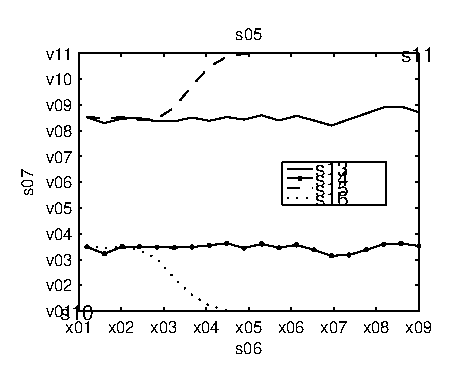
\includegraphics[width=\linewidth]{images/mean_error_z_bus}
  \caption[Time difference, method comparison. Mean error. $\hat{z}$-axis. (Bus)]{Comparison between traditional and matched filter methods. The vehicle was a bus. Mean error versus SNR. The sensor is placed 1.5 m from the vehicle and on the road surface. The sensor output in $\hat{z}$-axis has been used.}
  \label{fig:comp_mean_z_bus}
  \end{minipage}\hfill
  \begin{minipage}{0.45\linewidth}
   \centering
   % % generated by laprint.m
% %
% \begin{psfrags}%
% \psfragscanon%
% %
% text strings:
\psfrag{s05}[b][b]{\fontsize{8}{12}\fontseries{m}\mathversion{normal}\fontshape{n}\selectfont \setlength{\tabcolsep}{0pt}\begin{tabular}{c}Comparison between time difference methods\end{tabular}}%
\psfrag{s06}[t][t]{\fontsize{8}{12}\fontseries{m}\mathversion{normal}\fontshape{n}\selectfont \setlength{\tabcolsep}{0pt}\begin{tabular}{c}SNR [dB]\end{tabular}}%
\psfrag{s07}[b][b]{\fontsize{8}{12}\fontseries{m}\mathversion{normal}\fontshape{n}\selectfont \setlength{\tabcolsep}{0pt}\begin{tabular}{c}Error standard deviation [samples]\end{tabular}}%
\psfrag{s10}[][]{\fontsize{8}{12}\fontseries{m}\mathversion{normal}\fontshape{n}\selectfont \setlength{\tabcolsep}{0pt}\begin{tabular}{c} \end{tabular}}%
\psfrag{s11}[][]{\fontsize{4}{6}\fontseries{m}\mathversion{normal}\fontshape{n}\selectfont \setlength{\tabcolsep}{0pt}\begin{tabular}{c} \end{tabular}}%
\psfrag{s12}[l][l]{\fontsize{4}{6}\fontseries{m}\mathversion{normal}\fontshape{n}\selectfont MF LP}%
\psfrag{s13}[l][l]{\fontsize{4}{6}\fontseries{m}\mathversion{normal}\fontshape{n}\selectfont P-P}%
\psfrag{s14}[l][l]{\fontsize{4}{6}\fontseries{m}\mathversion{normal}\fontshape{n}\selectfont P-P LP}%
\psfrag{s15}[l][l]{\fontsize{4}{6}\fontseries{m}\mathversion{normal}\fontshape{n}\selectfont MF}%
\psfrag{s16}[l][l]{\fontsize{4}{6}\fontseries{m}\mathversion{normal}\fontshape{n}\selectfont MF LP}%
%
% axes font properties:
\fontsize{6}{8}\fontseries{m}\mathversion{normal}%
\fontshape{n}\selectfont%
%
% xticklabels:
\psfrag{x01}[t][t]{$0$}%
\psfrag{x02}[t][t]{$5$}%
\psfrag{x03}[t][t]{$10$}%
\psfrag{x04}[t][t]{$15$}%
\psfrag{x05}[t][t]{$20$}%
\psfrag{x06}[t][t]{$25$}%
\psfrag{x07}[t][t]{$30$}%
\psfrag{x08}[t][t]{$35$}%
\psfrag{x09}[t][t]{$40$}%
%
% yticklabels:
\psfrag{v01}[r][r]{$0$}%
\psfrag{v02}[r][r]{$0.2$}%
\psfrag{v03}[r][r]{$0.4$}%
\psfrag{v04}[r][r]{$0.6$}%
\psfrag{v05}[r][r]{$0.8$}%
\psfrag{v06}[r][r]{$1$}%
\psfrag{v07}[r][r]{$1.2$}%
\psfrag{v08}[r][r]{$1.4$}%
\psfrag{v09}[r][r]{$1.6$}%
\psfrag{v10}[r][r]{$1.8$}%
\psfrag{v11}[r][r]{$2$}%
% %
% % Figure:
% \resizebox{6cm}{!}{\includegraphics{std_error_z.eps}}%
% \end{psfrags}%
%
% End std_error_z.tex

   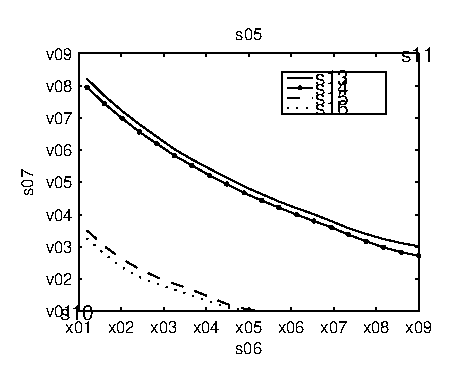
\includegraphics[width=\linewidth]{images/std_error_z_bus}
  \caption[Time difference, method comparison. Error standard deviation. $\hat{z}$-axis. (Bus)]{Comparison between traditional and matched filter methods. The vehicle was a bus. Standard deviation versus SNR. The sensor is placed 1.5 m from the vehicle and on the road surface. The sensor output in $\hat{z}$-axis has been used.}
  \label{fig:comp_std_z_bus}
  \end{minipage}
 \end{figure}
\end{subfigures}

\begin{subfigures}
\begin{figure}[!tbh]
  \centering
  \begin{minipage}{0.45\linewidth}
  \centering
  % generated by laprint.m
%
% \begin{psfrags}%
% \psfragscanon%
%
% text strings:
\psfrag{s05}[b][b]{\fontsize{8}{12}\fontseries{m}\mathversion{normal}\fontshape{n}\selectfont \setlength{\tabcolsep}{0pt}\begin{tabular}{c}Comparison between time difference methods\end{tabular}}%
\psfrag{s06}[t][t]{\fontsize{8}{12}\fontseries{m}\mathversion{normal}\fontshape{n}\selectfont \setlength{\tabcolsep}{0pt}\begin{tabular}{c}SNR [dB]\end{tabular}}%
\psfrag{s07}[b][b]{\fontsize{8}{12}\fontseries{m}\mathversion{normal}\fontshape{n}\selectfont \setlength{\tabcolsep}{0pt}\begin{tabular}{c}Mean error [samples]\end{tabular}}%
\psfrag{s10}[][]{\fontsize{8}{12}\fontseries{m}\mathversion{normal}\fontshape{n}\selectfont \setlength{\tabcolsep}{0pt}\begin{tabular}{c} \end{tabular}}%
\psfrag{s11}[][]{\fontsize{4}{6}\fontseries{m}\mathversion{normal}\fontshape{n}\selectfont \setlength{\tabcolsep}{0pt}\begin{tabular}{c} \end{tabular}}%
\psfrag{s12}[l][l]{\fontsize{4}{6}\fontseries{m}\mathversion{normal}\fontshape{n}\selectfont MF LP}%
\psfrag{s13}[l][l]{\fontsize{4}{6}\fontseries{m}\mathversion{normal}\fontshape{n}\selectfont P-P}%
\psfrag{s14}[l][l]{\fontsize{4}{6}\fontseries{m}\mathversion{normal}\fontshape{n}\selectfont P-P LP}%
\psfrag{s15}[l][l]{\fontsize{4}{6}\fontseries{m}\mathversion{normal}\fontshape{n}\selectfont MF}%
\psfrag{s16}[l][l]{\fontsize{4}{6}\fontseries{m}\mathversion{normal}\fontshape{n}\selectfont MF LP}%
%
% axes font properties:
\fontsize{6}{8}\fontseries{m}\mathversion{normal}%
\fontshape{n}\selectfont%
%
% xticklabels:
\psfrag{x01}[t][t]{$0$}%
\psfrag{x02}[t][t]{$5$}%
\psfrag{x03}[t][t]{$10$}%
\psfrag{x04}[t][t]{$15$}%
\psfrag{x05}[t][t]{$20$}%
\psfrag{x06}[t][t]{$25$}%
\psfrag{x07}[t][t]{$30$}%
\psfrag{x08}[t][t]{$35$}%
\psfrag{x09}[t][t]{$40$}%
%
% yticklabels:
\psfrag{v01}[r][r]{$0$}%
\psfrag{v02}[r][r]{$0.1$}%
\psfrag{v03}[r][r]{$0.2$}%
\psfrag{v04}[r][r]{$0.3$}%
\psfrag{v05}[r][r]{$0.4$}%
\psfrag{v06}[r][r]{$0.5$}%
\psfrag{v07}[r][r]{$0.6$}%
\psfrag{v08}[r][r]{$0.7$}%
\psfrag{v09}[r][r]{$0.8$}%
\psfrag{v10}[r][r]{$0.9$}%
\psfrag{v11}[r][r]{$1$}%
% %
% % Figure:
% \resizebox{6cm}{!}{\includegraphics{mean_error_r.eps}}%
% \end{psfrags}%
% %
% End mean_error_r.tex

   \includegraphics[width=\linewidth]{images/mean_error_r}
  \caption[Time difference, method comparison. Mean error. Norm.]{Comparison between traditional and matched filter methods. Mean error versus SNR. The sensor is placed 1.5 m from the vehicle and on the road surface. The norm of the sensor output has been used.}
  \label{fig:comp_mean_r}
  \end{minipage}\hfill
  \begin{minipage}{0.45\linewidth}
   \centering
   % % generated by laprint.m
% %
% \begin{psfrags}%
% \psfragscanon%
%
% text strings:
\psfrag{s05}[b][b]{\fontsize{8}{12}\fontseries{m}\mathversion{normal}\fontshape{n}\selectfont \setlength{\tabcolsep}{0pt}\begin{tabular}{c}Comparison between time difference methods\end{tabular}}%
\psfrag{s06}[t][t]{\fontsize{8}{12}\fontseries{m}\mathversion{normal}\fontshape{n}\selectfont \setlength{\tabcolsep}{0pt}\begin{tabular}{c}SNR [dB]\end{tabular}}%
\psfrag{s07}[b][b]{\fontsize{8}{12}\fontseries{m}\mathversion{normal}\fontshape{n}\selectfont \setlength{\tabcolsep}{0pt}\begin{tabular}{c}Error standard deviation [samples]\end{tabular}}%
\psfrag{s10}[][]{\fontsize{8}{12}\fontseries{m}\mathversion{normal}\fontshape{n}\selectfont \setlength{\tabcolsep}{0pt}\begin{tabular}{c} \end{tabular}}%
\psfrag{s11}[][]{\fontsize{4}{6}\fontseries{m}\mathversion{normal}\fontshape{n}\selectfont \setlength{\tabcolsep}{0pt}\begin{tabular}{c} \end{tabular}}%
\psfrag{s12}[l][l]{\fontsize{4}{6}\fontseries{m}\mathversion{normal}\fontshape{n}\selectfont MF LP}%
\psfrag{s13}[l][l]{\fontsize{4}{6}\fontseries{m}\mathversion{normal}\fontshape{n}\selectfont P-P}%
\psfrag{s14}[l][l]{\fontsize{4}{6}\fontseries{m}\mathversion{normal}\fontshape{n}\selectfont P-P LP}%
\psfrag{s15}[l][l]{\fontsize{4}{6}\fontseries{m}\mathversion{normal}\fontshape{n}\selectfont MF}%
\psfrag{s16}[l][l]{\fontsize{4}{6}\fontseries{m}\mathversion{normal}\fontshape{n}\selectfont MF LP}%
%
% axes font properties:
\fontsize{6}{8}\fontseries{m}\mathversion{normal}%
\fontshape{n}\selectfont%
%
% xticklabels:
\psfrag{x01}[t][t]{$0$}%
\psfrag{x02}[t][t]{$5$}%
\psfrag{x03}[t][t]{$10$}%
\psfrag{x04}[t][t]{$15$}%
\psfrag{x05}[t][t]{$20$}%
\psfrag{x06}[t][t]{$25$}%
\psfrag{x07}[t][t]{$30$}%
\psfrag{x08}[t][t]{$35$}%
\psfrag{x09}[t][t]{$40$}%
%
% yticklabels:
\psfrag{v01}[r][r]{$0$}%
\psfrag{v02}[r][r]{$0.2$}%
\psfrag{v03}[r][r]{$0.4$}%
\psfrag{v04}[r][r]{$0.6$}%
\psfrag{v05}[r][r]{$0.8$}%
\psfrag{v06}[r][r]{$1$}%
\psfrag{v07}[r][r]{$1.2$}%
\psfrag{v08}[r][r]{$1.4$}%
\psfrag{v09}[r][r]{$1.6$}%
\psfrag{v10}[r][r]{$1.8$}%
\psfrag{v11}[r][r]{$2$}%
%
% % Figure:
% \resizebox{6cm}{!}{\includegraphics{std_error_r.eps}}%
% \end{psfrags}%
% %
% End std_error_r.tex

   \includegraphics[width=\linewidth]{images/std_error_r}
  \caption[Time difference, method comparison. Error standard deviation. Norm.]{Comparison between traditional and matched filter methods. Standard deviation versus SNR. The sensor is placed 1.5 m from the vehicle and on the road surface. The norm of the sensor output has been used.}
  \label{fig:comp_std_r}
  \end{minipage}
 \end{figure}
\end{subfigures}

\begin{subfigures}
\begin{figure}[!tbh]
  \centering
  \begin{minipage}{0.45\linewidth}
  \centering
  % generated by laprint.m
% %
% \begin{psfrags}%
% \psfragscanon%
%
% text strings:
\psfrag{s05}[t][t]{\fontsize{8}{12}\fontseries{m}\mathversion{normal}\fontshape{n}\selectfont \setlength{\tabcolsep}{0pt}\begin{tabular}{c}Vehicle speed [km/h]\end{tabular}}%
\psfrag{s06}[b][b]{\fontsize{8}{12}\fontseries{m}\mathversion{normal}\fontshape{n}\selectfont \setlength{\tabcolsep}{0pt}\begin{tabular}{c}Mean error [samples]\end{tabular}}%
\psfrag{s08}[b][b]{\fontsize{8}{12}\fontseries{m}\mathversion{normal}\fontshape{n}\selectfont \setlength{\tabcolsep}{0pt}\begin{tabular}{c}Comparison between time difference methods\end{tabular}}%
\psfrag{s10}[][]{\fontsize{8}{12}\fontseries{m}\mathversion{normal}\fontshape{n}\selectfont \setlength{\tabcolsep}{0pt}\begin{tabular}{c} \end{tabular}}%
\psfrag{s11}[][]{\fontsize{4}{6}\fontseries{m}\mathversion{normal}\fontshape{n}\selectfont \setlength{\tabcolsep}{0pt}\begin{tabular}{c} \end{tabular}}%
\psfrag{s12}[l][l]{\fontsize{4}{6}\fontseries{m}\mathversion{normal}\fontshape{n}\selectfont MF LP}%
\psfrag{s13}[l][l]{\fontsize{4}{6}\fontseries{m}\mathversion{normal}\fontshape{n}\selectfont P-P}%
\psfrag{s14}[l][l]{\fontsize{4}{6}\fontseries{m}\mathversion{normal}\fontshape{n}\selectfont P-P LP}%
\psfrag{s15}[l][l]{\fontsize{4}{6}\fontseries{m}\mathversion{normal}\fontshape{n}\selectfont MF}%
\psfrag{s16}[l][l]{\fontsize{4}{6}\fontseries{m}\mathversion{normal}\fontshape{n}\selectfont MF LP}%
%
% axes font properties:
\fontsize{6}{8}\fontseries{m}\mathversion{normal}%
\fontshape{n}\selectfont%
%
% xticklabels:
\psfrag{x01}[t][t]{$0$}%
\psfrag{x02}[t][t]{$20$}%
\psfrag{x03}[t][t]{$40$}%
\psfrag{x04}[t][t]{$60$}%
\psfrag{x05}[t][t]{$80$}%
\psfrag{x06}[t][t]{$100$}%
\psfrag{x07}[t][t]{$120$}%
%
% yticklabels:
\psfrag{v01}[r][r]{$-1$}%
\psfrag{v02}[r][r]{$-0.8$}%
\psfrag{v03}[r][r]{$-0.6$}%
\psfrag{v04}[r][r]{$-0.4$}%
\psfrag{v05}[r][r]{$-0.2$}%
\psfrag{v06}[r][r]{$0$}%
\psfrag{v07}[r][r]{$0.2$}%
\psfrag{v08}[r][r]{$0.4$}%
\psfrag{v09}[r][r]{$0.6$}%
\psfrag{v10}[r][r]{$0.8$}%
\psfrag{v11}[r][r]{$1$}%
%
% % Figure:
% \resizebox{6cm}{!}{\includegraphics{mean_error-velocity.eps}}%
% \end{psfrags}%
% %
% End mean_error-velocity.tex

   \includegraphics[width=\linewidth]{images/mean_error-velocity}
  \caption[Time difference, method comparison. Mean error versus velocity]{Comparison between traditional and matched filter methods. Mean error versus velocity. The sensor is placed 1.5 m from the vehicle and on the road surface. The sensor output in $\hat{z}$-axis has been used.}
  \label{fig:comp_mean-vel}
  \end{minipage}\hfill
  \begin{minipage}{0.45\linewidth}
   \centering
   % generated by laprint.m
%
% \begin{psfrags}%
% \psfragscanon%
%
% text strings:
\psfrag{s05}[b][b]{\fontsize{8}{12}\fontseries{m}\mathversion{normal}\fontshape{n}\selectfont \setlength{\tabcolsep}{0pt}\begin{tabular}{c}Comparison between time difference methods\end{tabular}}%
\psfrag{s06}[t][t]{\fontsize{8}{12}\fontseries{m}\mathversion{normal}\fontshape{n}\selectfont \setlength{\tabcolsep}{0pt}\begin{tabular}{c}Vehicle speed [km/h]\end{tabular}}%
\psfrag{s07}[b][b]{\fontsize{8}{12}\fontseries{m}\mathversion{normal}\fontshape{n}\selectfont \setlength{\tabcolsep}{0pt}\begin{tabular}{c}Error standard deviation [samples]\end{tabular}}%
\psfrag{s10}[][]{\fontsize{8}{12}\fontseries{m}\mathversion{normal}\fontshape{n}\selectfont \setlength{\tabcolsep}{0pt}\begin{tabular}{c} \end{tabular}}%
\psfrag{s11}[][]{\fontsize{4}{6}\fontseries{m}\mathversion{normal}\fontshape{n}\selectfont \setlength{\tabcolsep}{0pt}\begin{tabular}{c} \end{tabular}}%
\psfrag{s12}[l][l]{\fontsize{4}{6}\fontseries{m}\mathversion{normal}\fontshape{n}\selectfont MF LP}%
\psfrag{s13}[l][l]{\fontsize{4}{6}\fontseries{m}\mathversion{normal}\fontshape{n}\selectfont P-P}%
\psfrag{s14}[l][l]{\fontsize{4}{6}\fontseries{m}\mathversion{normal}\fontshape{n}\selectfont P-P LP}%
\psfrag{s15}[l][l]{\fontsize{4}{6}\fontseries{m}\mathversion{normal}\fontshape{n}\selectfont MF}%
\psfrag{s16}[l][l]{\fontsize{4}{6}\fontseries{m}\mathversion{normal}\fontshape{n}\selectfont MF LP}%
%
% axes font properties:
\fontsize{6}{8}\fontseries{m}\mathversion{normal}%
\fontshape{n}\selectfont%
%
% xticklabels:
\psfrag{x01}[t][t]{$0$}%
\psfrag{x02}[t][t]{$20$}%
\psfrag{x03}[t][t]{$40$}%
\psfrag{x04}[t][t]{$60$}%
\psfrag{x05}[t][t]{$80$}%
\psfrag{x06}[t][t]{$100$}%
\psfrag{x07}[t][t]{$120$}%
%
% yticklabels:
\psfrag{v01}[r][r]{$0$}%
\psfrag{v02}[r][r]{$0.5$}%
\psfrag{v03}[r][r]{$1$}%
\psfrag{v04}[r][r]{$1.5$}%
\psfrag{v05}[r][r]{$2$}%
\psfrag{v06}[r][r]{$2.5$}%
%
% Figure:
% \resizebox{6cm}{!}{\includegraphics{std_error-velocity.eps}}%
% \end{psfrags}%
%
% End std_error-velocity.tex

   \includegraphics[width=\linewidth]{images/std_error-velocity}
  \caption[Time difference, method comparison. Error standard deviation versus velocity]{Comparison between traditional and matched filter methods. Standard deviation versus velocity. The sensor is placed 1.5 m from the vehicle and on the road surface. The sensor output in $\hat{z}$-axis has been used.}
  \label{fig:comp_std-vel}
  \end{minipage}
 \end{figure}
\end{subfigures}

Peak-to-peak\index{Peak-to-peak} time difference has a higher mean error than the matched filter method for low noise situations. We can see in \mbox{Figure \ref{fig:comp_mean_z}} how the lowpass filter introduces a delay. Both methods has the same error in case of high noise. P-P has a much higher standard deviation than using matched filter. We can see how the LP filter reduces standard deviation in both cases but not by much. The recommendation is to use matched filter without LP filter.

The benefit of using the matched filter method is clearly better estimation of the time difference. However, the disadvantage of this method is that the matched filter requires knowledge of both signals and therefore more information has to be sent over the network. We should note that these calculations can be done in close to real-time, and the decision can be taken when the vehicle has passed both sensors.

With a more complex signal, as seen in Figures~\ref{fig:comp_mean_z_bus} and \ref{fig:comp_std_z_bus} the error goes to zero faster for the matched filter method. This means that we should choose the most complex axis or a combination of axes when using this algorithm. We can also see that since a higher vehicle velocity will give us sharper peaks, the error becomes smaller with greater speeds. The standard deviation also becomes smaller. Note that graphs are plotted versus SNR and that the signal amplitude is different for different vehicles and axes.

One important aspect of this algorithm is that it is not affected by the difference in sensitivity\index{sensitivity} as the traditional algorithm is.

The SNR is defined as
\begin{equation}
 \lfloor{}\text{SNR}\rfloor_{\text{dB}} = 10 \log{\left(\frac{\left\langle{}x^2(t)\right\rangle}{\sigma^2}\right)},
\end{equation}
where $\left\langle{}x^2(t)\right\rangle$ is the mean of the square of our signal as
\begin{equation}
  \left\langle{}x^2(t)\right\rangle = \frac{1}{n} \sum_{i=1}^{n} x_i^2,
\end{equation}
 if $x_i(t)$ is a discrete function with $n$ samples. $\sigma$ is the standard deviation of the Gaussian noise. For the plots in this section, the SNR of the signal from the first sensor has been used. If we have used another reference signal, we will get $\left\langle{}x_1^2(t)\right\rangle = \alpha\left\langle{}x_2^2(t)\right\rangle$ where $\alpha$ is a factor. Due to the nature of logarithms, this will only introduce an offset.

If sensors are placed in pairs with one master and one slave, the master is responsible for uploading the measured data to the system. Due to the asymmetric power consumption between master and slave, it might be better to upload all data to the access point before processing.

\subsection{Average speed estimations}\label{sec:avg_per}\index{speed estimation!average vehicle}

A simulation result of the occupancy method can be seen in \mbox{Figure \ref{fig:occSpeedHist}}. We can deduce from the histogram that the standard deviation is quite large for this method.

\begin{figure}
 \centering
 \begin{minipage}{0.45\linewidth}
 \centering
 % generated by laprint.m
%
% \begin{psfrags}%
% \psfragscanon%
%
% text strings:
\psfrag{s02}[t][t]{\fontsize{8}{12}\fontseries{m}\mathversion{normal}\fontshape{n}\selectfont \setlength{\tabcolsep}{0pt}\begin{tabular}{c}Speed [km/h]\end{tabular}}%
\psfrag{s03}[b][b]{\fontsize{8}{12}\fontseries{m}\mathversion{normal}\fontshape{n}\selectfont \setlength{\tabcolsep}{0pt}\begin{tabular}{c}Number of vehicles\end{tabular}}%
\psfrag{s04}[b][b]{\fontsize{8}{12}\fontseries{m}\mathversion{normal}\fontshape{n}\selectfont \setlength{\tabcolsep}{0pt}\begin{tabular}{c}Distribution of vehicle speed\end{tabular}}%
%
% axes font properties:
\fontsize{6}{12}\fontseries{m}\mathversion{normal}%
\fontshape{n}\selectfont%
%
% xticklabels:
\psfrag{x01}[t][t]{$0$}%
\psfrag{x02}[t][t]{$50$}%
\psfrag{x03}[t][t]{$100$}%
\psfrag{x04}[t][t]{$150$}%
\psfrag{x05}[t][t]{$200$}%
\psfrag{x06}[t][t]{$250$}%
\psfrag{x07}[t][t]{$300$}%
\psfrag{x08}[t][t]{$350$}%
\psfrag{x09}[t][t]{$400$}%
%
% yticklabels:
\psfrag{v01}[r][r]{$0$}%
\psfrag{v02}[r][r]{$200$}%
\psfrag{v03}[r][r]{$400$}%
\psfrag{v04}[r][r]{$600$}%
\psfrag{v05}[r][r]{$800$}%
\psfrag{v06}[r][r]{$1000$}%
\psfrag{v07}[r][r]{$1200$}%
%
% Figure:
% \resizebox{6cm}{!}{\includegraphics{occupancSpeedHist.eps}}%
% \end{psfrags}%
%
% End occupancSpeedHist.tex

 \includegraphics[width=1\linewidth]{images/occupancSpeedHist}
 \caption[Estimated speed using the occupancy method.]{Estimated speed using the occupancy method from Section \ref{sec:avg}. True speed was \mbox{72~km/h} and only passenger cars were used. Mean speed was \mbox{$78.6$~km/h} and median speed was \mbox{$60.4$ km/h}. Vehicles with speed over \mbox{360~km/h} was discarded. The total number of remaining vehicles was 8642 and $\hat{l}$ was chosen to be \mbox{4.5~m}. Adjusting this parameter will shift the distribution. The time interval was 10 seconds.}
 \label{fig:occSpeedHist}
 \end{minipage}
\hfill
 \begin{minipage}{0.45\linewidth}
 \centering
 % generated by laprint.m
% %
% \begin{psfrags}%
% \psfragscanon%
% %
% text strings:
\psfrag{s02}[b][b]{\fontsize{8}{12}\fontseries{m}\mathversion{normal}\fontshape{n}\selectfont \setlength{\tabcolsep}{0pt}\begin{tabular}{c}Distribution of vehicle median speed\end{tabular}}%
\psfrag{s03}[t][t]{\fontsize{8}{12}\fontseries{m}\mathversion{normal}\fontshape{n}\selectfont \setlength{\tabcolsep}{0pt}\begin{tabular}{c}Speed [km/h]\end{tabular}}%
\psfrag{s04}[b][b]{\fontsize{8}{12}\fontseries{m}\mathversion{normal}\fontshape{n}\selectfont \setlength{\tabcolsep}{0pt}\begin{tabular}{c}Number of vehicles\end{tabular}}%
%
% axes font properties:
\fontsize{6}{8}\fontseries{m}\mathversion{normal}%
\fontshape{n}\selectfont%
%
% xticklabels:
\psfrag{x01}[t][t]{$30$}%
\psfrag{x02}[t][t]{$40$}%
\psfrag{x03}[t][t]{$50$}%
\psfrag{x04}[t][t]{$60$}%
\psfrag{x05}[t][t]{$70$}%
\psfrag{x06}[t][t]{$80$}%
\psfrag{x07}[t][t]{$90$}%
%
% yticklabels:
\psfrag{v01}[r][r]{$0$}%
\psfrag{v02}[r][r]{$200$}%
\psfrag{v03}[r][r]{$400$}%
\psfrag{v04}[r][r]{$600$}%
\psfrag{v05}[r][r]{$800$}%
\psfrag{v06}[r][r]{$1000$}%
\psfrag{v07}[r][r]{$1200$}%
\psfrag{v08}[r][r]{$1400$}%
\psfrag{v09}[r][r]{$1600$}%
\psfrag{v10}[r][r]{$1800$}%
\psfrag{v11}[r][r]{$2000$}%
%
% Figure:
% \resizebox{6cm}{!}{\includegraphics{speedmed_hist.eps}}%
% \end{psfrags}%
%
% End speedmed_hist.tex

 \includegraphics[width=1\linewidth]{images/speedmed_hist}
 \caption[Estimated speed using the median velocity method.]{Estimated speed using the median velocity method from Section \ref{sec:avg}. The true speed was \mbox{72 km/h}, mean speed was \mbox{$73.8$~km/h} and the median speed was \mbox{$77.1$~km/h}. Standard deviation was \mbox{$8.95$~km/h}. The total number of vehicles was above 3000. $\hat{l}$ was chosen to be \mbox{4.5 m}. Adjusting this parameter will shift the distribution. Note the over estimation due to $\hat{l}$ and the shape of the distribution.\\}
 \label{fig:speedmed_hist}
 \end{minipage}
\end{figure}

In Figure~\ref{fig:speedmed_hist} we can see the result from the median speed method. The fact that the method over estimates the speed can be corrected for by adjusting the $\hat{l}$ parameter. The standard deviation was \mbox{$8.95$~km/h} or \mbox{$5.57$~mph} which is somewhat larger than the reported $2.5$~mph standard deviation for a 10-point median speed estimation in~\cite{cheung2005-2}.
% \begin{subfigures}
% \begin{figure}[!ht]
%   \centering
%   \begin{minipage}{0.45\linewidth}
%   \centering
%    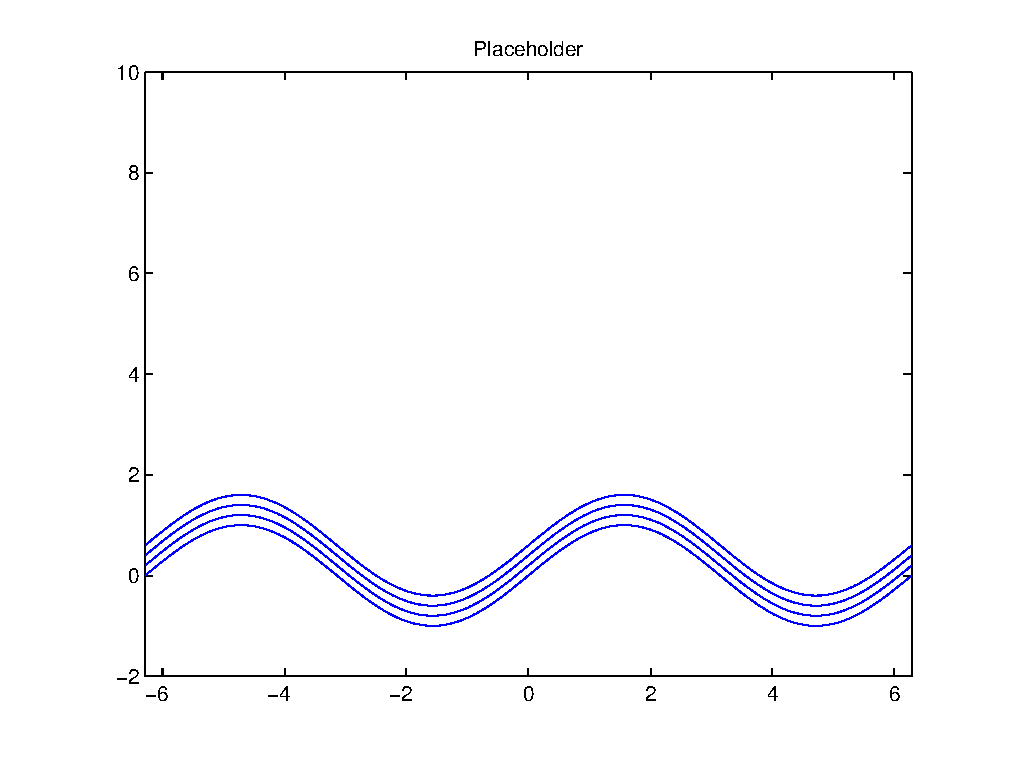
\includegraphics[width=\linewidth]{images/placeholder}
%   \caption[Median of vehicle speed. Sensor at the side of the road]{5-point and 11-point median of vehicle speed. Sensor node is placed at the side of the road.}
%   \label{fig:medianspeed_side}
%   \end{minipage}\hfill
%   \begin{minipage}{0.45\linewidth}
%    \centering
%    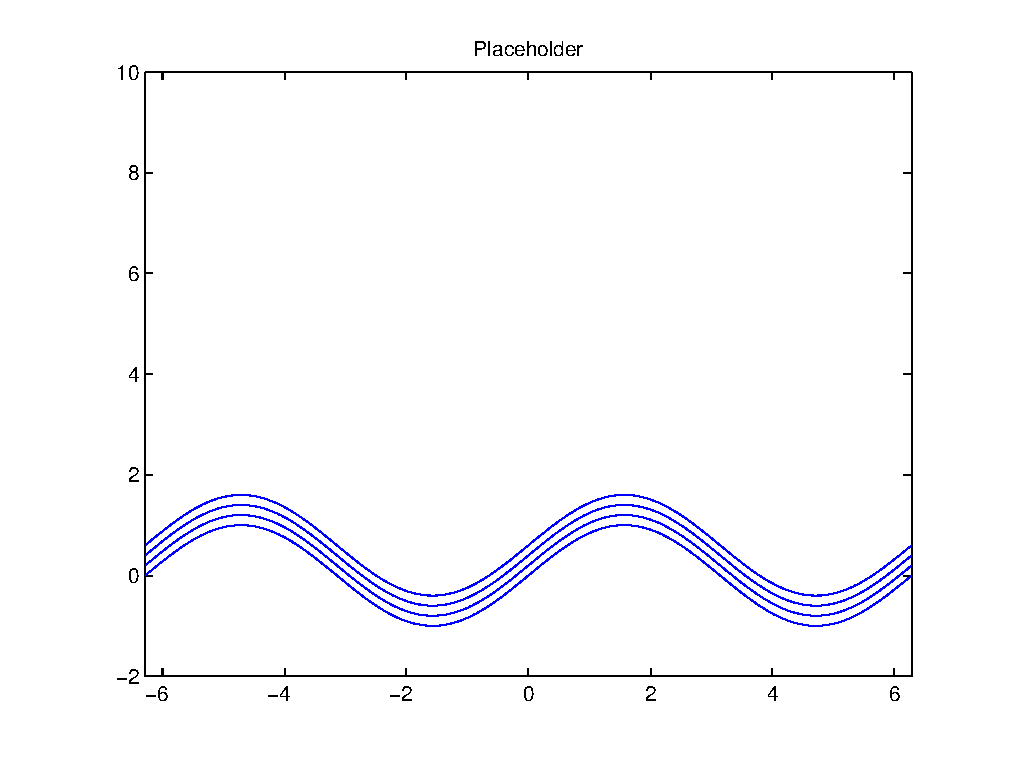
\includegraphics[width=\linewidth]{images/placeholder}
%   \caption[Median of vehicle length. Sensor at the side of the road]{5-point and 11-point median of vehicle length. Sensor node is placed at the side of the road.}
%   \label{fig:medianlength_side}
%   \end{minipage}
%  \end{figure}
% \end{subfigures}


% \begin{subfigures}
% \begin{figure}[!ht]
%   \centering
%   \begin{minipage}{0.45\linewidth}
%   \centering
%    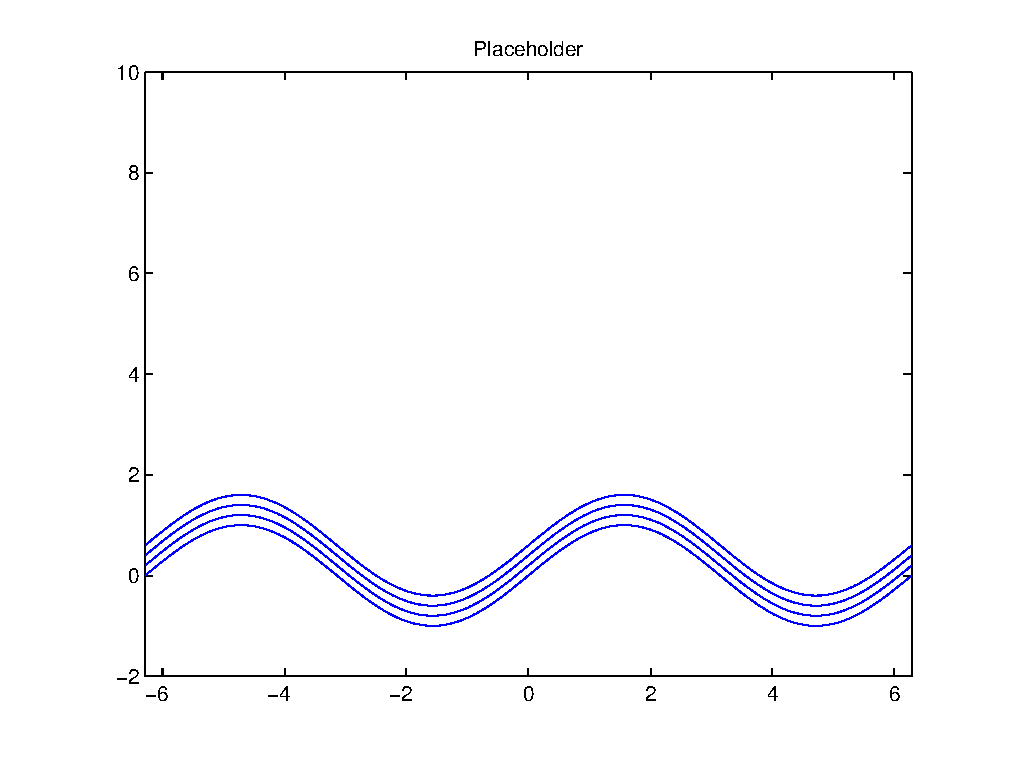
\includegraphics[width=\linewidth]{images/placeholder}
%   \caption[Median of vehicle speed. Sensor in middle of lane]{5-point and 11-point median of vehicle speed. Sensor node is placed at the middle of the lane.}
%   \label{fig:medianspeed_middle}
%   \end{minipage}\hfill
%   \begin{minipage}{0.45\linewidth}
%    \centering
%    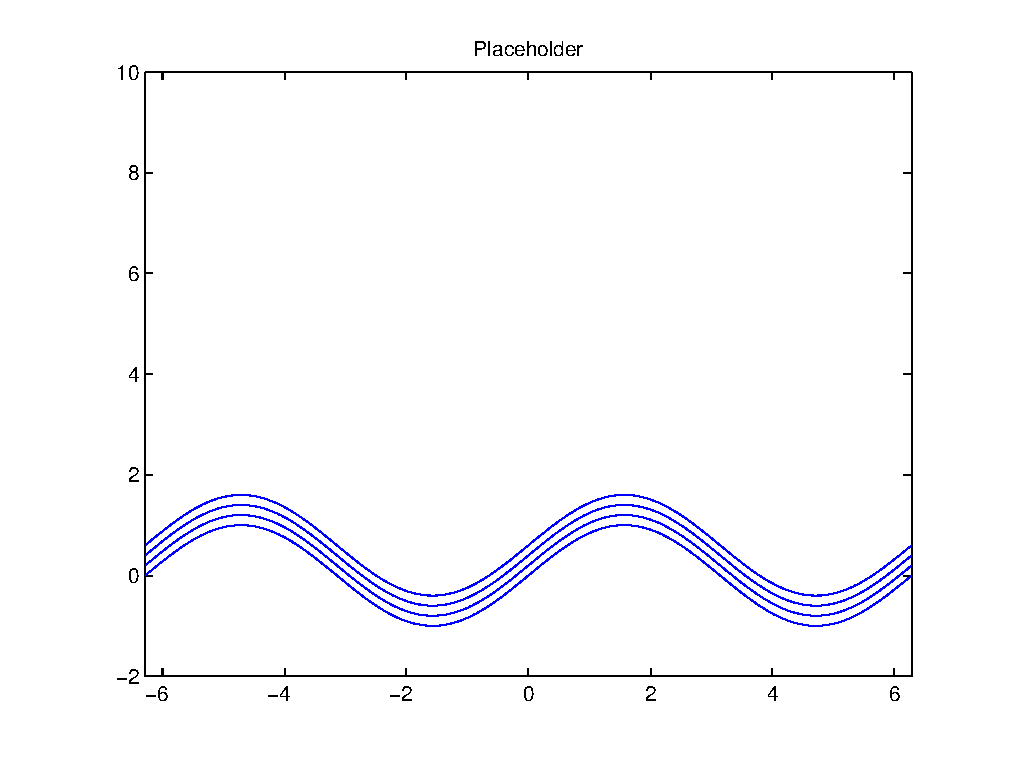
\includegraphics[width=\linewidth]{images/placeholder}
%   \caption[Median of vehicle length. Sensor in middle of lane]{5-point and 11-point median of vehicle length. Sensor node is placed at the middle of the lane.}
%   \label{fig:medianlength_middle}
%   \end{minipage}
%  \end{figure}
% \end{subfigures}

\section{Classification}\index{classification}

The classification schemes are very different depending on sensor positions. In the limited simulations done we have found the classification rate to be nearly 100~\% when the sensor is placed in the roadway. The classification has been done in three classes; Passenger cars, SUVs (high cars) and buses. A classification accuracy of 60~\% has been reported~\cite{cheung2005-2} not using length as a feature. Using the two sensors in a pair will of course make the classification more accurate, especially since we then can use the speed estimation to estimate the vehicle length.

Since it is expensive to install sensors in the roadway, we have decided to only use sensors at the side of the road. A roadside sensor position make classification much more difficult. Due to the signature properties, we can use the derivative of the signal to increase the accuracy. This method is more sensitive to noise, and requires filtering of the signal.

We can also look at the transform of the signal, for example the FFT. The FFT of different vehicle signatures can be seen in Appendix~\ref{chap:plots}. These transformed signals show potential to be used for classification, although it will need further investigation.

\subsection{Estimation of model parameters}\index{least-squares estimation}\label{sec:leastsq_per}

One method of classification is trying to estimate the parameters that we use in our model, and compare the results to our database of vehicles. The database that we are using does not contain enough data to give a good analysis of the relability of the method but we can use the method for a proof of concept.

When using the least-squares estimation method described in Section~\ref{subsec:leastsq} we obtain the results than can be seen in Figure~\ref{fig-leastsqest}. The measured data can be seen in Figure~\ref{fig-leastsqdata}.

The parameters estimated are as earlier stated
\begin{align}
	\vec{\mu}_i &= \left[\,\mu_{x,i}\quad{}\mu_{y,i}\quad{}\mu_{z,i}\,\right]\\
	\vec{r}_i &= \left[\,x_i\quad{}y_i\quad{}z_i\,\right].
\end{align}
It is assumed that the magnetic moments will lie on a straight line in the center of the vehicle thereby eliminating two degrees of freedom. The vehicle is furthermore assumed to be travelling a straight path perpendicular to the sensor. Since the vehicle coordinate system will move, we can add the speed $v$ as another parameter. In all, twelve parameters are estimated from measurements.

The estimated data and measured data almost match in shape, but not in amplitude. The most interesting thing we can see from this estimation is that in an estimation of three different magnetic moments for a passenger vehicle, two of the magnetic moments are very close in position and has opposite signs in at least two axes. This means that our model of using only one magnetic moment is probably a good model. An estimation with only one estimated magnetic moment can be seen in Figure~\ref{fig-est_data_one}. The discrepancy is in both estimation due to a number of unknown parameters in the measurements done by \textsc{Imego}, however we can still see the similarity. Among those parameters are the distance to the sensor and the vehicle velocity.

\begin{subfigures}
\begin{figure}[!htb]
  \centering
  \begin{minipage}{0.45\linewidth}
  \centering
   % % generated by laprint.m
% %
% \begin{psfrags}%
% \psfragscanon%
% %
% text strings:
\psfrag{s05}[t][t]{\fontsize{8}{12}\fontseries{m}\mathversion{normal}\fontshape{n}\selectfont \setlength{\tabcolsep}{0pt}\begin{tabular}{c}Time [s]\end{tabular}}%
\psfrag{s06}[b][b]{\fontsize{8}{12}\fontseries{m}\mathversion{normal}\fontshape{n}\selectfont \setlength{\tabcolsep}{0pt}\begin{tabular}{c}Magnetic field strength [nT]\end{tabular}}%
\psfrag{s07}[b][b]{\fontsize{8}{12}\fontseries{m}\mathversion{normal}\fontshape{n}\selectfont \setlength{\tabcolsep}{0pt}\begin{tabular}{c}Data from estimation\end{tabular}}%
\psfrag{s10}[][]{\fontsize{8}{12}\fontseries{m}\mathversion{normal}\fontshape{n}\selectfont \setlength{\tabcolsep}{0pt}\begin{tabular}{c} \end{tabular}}%
\psfrag{s11}[][]{\fontsize{8}{12}\fontseries{m}\mathversion{normal}\fontshape{n}\selectfont \setlength{\tabcolsep}{0pt}\begin{tabular}{c} \end{tabular}}%
\psfrag{s12}[l][l]{\fontsize{6}{8}\fontseries{m}\mathversion{normal}\fontshape{n}\selectfont $\hat{z}$}%
\psfrag{s13}[l][l]{\fontsize{6}{8}\fontseries{m}\mathversion{normal}\fontshape{n}\selectfont $\hat{x}$}%
\psfrag{s14}[l][l]{\fontsize{6}{8}\fontseries{m}\mathversion{normal}\fontshape{n}\selectfont $\hat{y}$}%
\psfrag{s15}[l][l]{\fontsize{6}{8}\fontseries{m}\mathversion{normal}\fontshape{n}\selectfont $\hat{z}$}%
%
% axes font properties:
\fontsize{6}{8}\fontseries{m}\mathversion{normal}%
\fontshape{n}\selectfont%
%
% xticklabels:
\psfrag{x01}[t][t]{$-0.5$}%
\psfrag{x02}[t][t]{$-0.4$}%
\psfrag{x03}[t][t]{$-0.3$}%
\psfrag{x04}[t][t]{$-0.2$}%
\psfrag{x05}[t][t]{$-0.1$}%
\psfrag{x06}[t][t]{$0$}%
\psfrag{x07}[t][t]{$0.1$}%
\psfrag{x08}[t][t]{$0.2$}%
\psfrag{x09}[t][t]{$0.3$}%
\psfrag{x10}[t][t]{$0.4$}%
\psfrag{x11}[t][t]{$0.5$}%
%
% yticklabels:
\psfrag{v01}[r][r]{$-500$}%
\psfrag{v02}[r][r]{$0$}%
\psfrag{v03}[r][r]{$500$}%
\psfrag{v04}[r][r]{$1000$}%
\psfrag{v05}[r][r]{$1500$}%
\psfrag{v06}[r][r]{$2000$}%
%
% % Figure:
% \resizebox{6cm}{!}{\includegraphics{meas_data_three.eps}}%
% \end{psfrags}%
% %
% End meas_data_three.tex

   \includegraphics[width=\linewidth]{images/meas_data_three}
  \caption[Data from estimated parameters, three magnetic moments]{Data from estimated parameters. Three magnetic moments were estimated. Note the different time scale.}
  \label{fig-leastsqdata}
  \end{minipage}\hfill
  \begin{minipage}{0.45\linewidth}
   \centering
     % generated by laprint.m
%
% \begin{psfrags}%
% \psfragscanon%
%
% text strings:
\psfrag{s05}[t][t]{\fontsize{8}{12}\fontseries{m}\mathversion{normal}\fontshape{n}\selectfont \setlength{\tabcolsep}{0pt}\begin{tabular}{c}Time [s]\end{tabular}}%
\psfrag{s06}[b][b]{\fontsize{8}{12}\fontseries{m}\mathversion{normal}\fontshape{n}\selectfont \setlength{\tabcolsep}{0pt}\begin{tabular}{c}Magnetic field strength [nT]\end{tabular}}%
\psfrag{s07}[b][b]{\fontsize{8}{12}\fontseries{m}\mathversion{normal}\fontshape{n}\selectfont \setlength{\tabcolsep}{0pt}\begin{tabular}{c}Measured data\end{tabular}}%
\psfrag{s10}[][]{\fontsize{8}{12}\fontseries{m}\mathversion{normal}\fontshape{n}\selectfont \setlength{\tabcolsep}{0pt}\begin{tabular}{c} \end{tabular}}%
\psfrag{s11}[][]{\fontsize{8}{12}\fontseries{m}\mathversion{normal}\fontshape{n}\selectfont \setlength{\tabcolsep}{0pt}\begin{tabular}{c} \end{tabular}}%
\psfrag{s12}[l][l]{\fontsize{6}{8}\fontseries{m}\mathversion{normal}\fontshape{n}\selectfont $\hat{z}$}%
\psfrag{s13}[l][l]{\fontsize{6}{8}\fontseries{m}\mathversion{normal}\fontshape{n}\selectfont $\hat{x}$}%
\psfrag{s14}[l][l]{\fontsize{6}{8}\fontseries{m}\mathversion{normal}\fontshape{n}\selectfont $\hat{y}$}%
\psfrag{s15}[l][l]{\fontsize{6}{8}\fontseries{m}\mathversion{normal}\fontshape{n}\selectfont $\hat{z}$}%
%
% axes font properties:
\fontsize{6}{8}\fontseries{m}\mathversion{normal}%
\fontshape{n}\selectfont%
%
% xticklabels:
\psfrag{x01}[t][t]{$-0.5$}%
\psfrag{x02}[t][t]{$-0.4$}%
\psfrag{x03}[t][t]{$-0.3$}%
\psfrag{x04}[t][t]{$-0.2$}%
\psfrag{x05}[t][t]{$-0.1$}%
\psfrag{x06}[t][t]{$0$}%
\psfrag{x07}[t][t]{$0.1$}%
\psfrag{x08}[t][t]{$0.2$}%
\psfrag{x09}[t][t]{$0.3$}%
\psfrag{x10}[t][t]{$0.4$}%
\psfrag{x11}[t][t]{$0.5$}%
%
% yticklabels:
\psfrag{v01}[r][r]{$-500$}%
\psfrag{v02}[r][r]{$0$}%
\psfrag{v03}[r][r]{$500$}%
\psfrag{v04}[r][r]{$1000$}%
\psfrag{v05}[r][r]{$1500$}%
\psfrag{v06}[r][r]{$2000$}%
%
% % Figure:
% \resizebox{6cm}{!}{\includegraphics{est_data_three.eps}}%
% \end{psfrags}%
%
% End est_data_three.tex

   \includegraphics[width=\linewidth]{images/est_data_three}
  \caption[Measured data from passing vehicle.]{Measured data from passing vehicle.\\}
  \label{fig-leastsqest}
  \end{minipage}
 \end{figure}
% \end{subfigures}

%  \begin{subfigures}
\begin{figure}[!htb]
  \centering
%   \begin{minipage}{0.45\linewidth}
%   \centering
%   % generated by laprint.m
% %
% \begin{psfrags}%
% \psfragscanon%
%
% text strings:
\psfrag{s05}[t][t]{\fontsize{8}{12}\fontseries{m}\mathversion{normal}\fontshape{n}\selectfont \setlength{\tabcolsep}{0pt}\begin{tabular}{c}Time [s]\end{tabular}}%
\psfrag{s06}[b][b]{\fontsize{8}{12}\fontseries{m}\mathversion{normal}\fontshape{n}\selectfont \setlength{\tabcolsep}{0pt}\begin{tabular}{c}Magnetic field strength [nT]\end{tabular}}%
\psfrag{s07}[b][b]{\fontsize{8}{12}\fontseries{m}\mathversion{normal}\fontshape{n}\selectfont \setlength{\tabcolsep}{0pt}\begin{tabular}{c}Data from estimation\end{tabular}}%
\psfrag{s10}[][]{\fontsize{8}{12}\fontseries{m}\mathversion{normal}\fontshape{n}\selectfont \setlength{\tabcolsep}{0pt}\begin{tabular}{c} \end{tabular}}%
\psfrag{s11}[][]{\fontsize{8}{12}\fontseries{m}\mathversion{normal}\fontshape{n}\selectfont \setlength{\tabcolsep}{0pt}\begin{tabular}{c} \end{tabular}}%
\psfrag{s12}[l][l]{\fontsize{6}{8}\fontseries{m}\mathversion{normal}\fontshape{n}\selectfont $\hat{z}$}%
\psfrag{s13}[l][l]{\fontsize{6}{8}\fontseries{m}\mathversion{normal}\fontshape{n}\selectfont $\hat{x}$}%
\psfrag{s14}[l][l]{\fontsize{6}{8}\fontseries{m}\mathversion{normal}\fontshape{n}\selectfont $\hat{y}$}%
\psfrag{s15}[l][l]{\fontsize{6}{8}\fontseries{m}\mathversion{normal}\fontshape{n}\selectfont $\hat{z}$}%
%
% axes font properties:
\fontsize{6}{8}\fontseries{m}\mathversion{normal}%
\fontshape{n}\selectfont%
%
% xticklabels:
\psfrag{x01}[t][t]{$-0.5$}%
\psfrag{x02}[t][t]{$-0.4$}%
\psfrag{x03}[t][t]{$-0.3$}%
\psfrag{x04}[t][t]{$-0.2$}%
\psfrag{x05}[t][t]{$-0.1$}%
\psfrag{x06}[t][t]{$0$}%
\psfrag{x07}[t][t]{$0.1$}%
\psfrag{x08}[t][t]{$0.2$}%
\psfrag{x09}[t][t]{$0.3$}%
\psfrag{x10}[t][t]{$0.4$}%
\psfrag{x11}[t][t]{$0.5$}%
%
% yticklabels:
\psfrag{v01}[r][r]{$-1000$}%
\psfrag{v02}[r][r]{$-500$}%
\psfrag{v03}[r][r]{$0$}%
\psfrag{v04}[r][r]{$500$}%
\psfrag{v05}[r][r]{$1000$}%
\psfrag{v06}[r][r]{$1500$}%
%
% % Figure:
% \resizebox{6cm}{!}{\includegraphics{meas_data_one.eps}}%
% \end{psfrags}%
%
% End meas_data_one.tex

%    \includegraphics[width=\linewidth]{images/meas_data_one}
%   \caption[Measured data from passing vehicle.]{Measured data from passing vehicle.}
%   \label{fig-meas_data_one}
%    \end{minipage}
% %  \end{figure}
%  \hfill
   \begin{minipage}{0.45\linewidth}
    \centering
    % generated by laprint.m
%
% \begin{psfrags}%
% \psfragscanon%
% %
% text strings:
\psfrag{s05}[t][t]{\fontsize{8}{12}\fontseries{m}\mathversion{normal}\fontshape{n}\selectfont \setlength{\tabcolsep}{0pt}\begin{tabular}{c}Time [s]\end{tabular}}%
\psfrag{s06}[b][b]{\fontsize{8}{12}\fontseries{m}\mathversion{normal}\fontshape{n}\selectfont \setlength{\tabcolsep}{0pt}\begin{tabular}{c}Magnetic field strength [nT]\end{tabular}}%
\psfrag{s07}[b][b]{\fontsize{8}{12}\fontseries{m}\mathversion{normal}\fontshape{n}\selectfont \setlength{\tabcolsep}{0pt}\begin{tabular}{c}Measured data\end{tabular}}%
\psfrag{s10}[][]{\fontsize{8}{12}\fontseries{m}\mathversion{normal}\fontshape{n}\selectfont \setlength{\tabcolsep}{0pt}\begin{tabular}{c} \end{tabular}}%
\psfrag{s11}[][]{\fontsize{8}{12}\fontseries{m}\mathversion{normal}\fontshape{n}\selectfont \setlength{\tabcolsep}{0pt}\begin{tabular}{c} \end{tabular}}%
\psfrag{s12}[l][l]{\fontsize{6}{8}\fontseries{m}\mathversion{normal}\fontshape{n}\selectfont $\hat{z}$}%
\psfrag{s13}[l][l]{\fontsize{6}{8}\fontseries{m}\mathversion{normal}\fontshape{n}\selectfont $\hat{x}$}%
\psfrag{s14}[l][l]{\fontsize{6}{8}\fontseries{m}\mathversion{normal}\fontshape{n}\selectfont $\hat{y}$}%
\psfrag{s15}[l][l]{\fontsize{6}{8}\fontseries{m}\mathversion{normal}\fontshape{n}\selectfont $\hat{z}$}%
%
% axes font properties:
\fontsize{6}{8}\fontseries{m}\mathversion{normal}%
\fontshape{n}\selectfont%
%
% xticklabels:
\psfrag{x01}[t][t]{$-0.5$}%
\psfrag{x02}[t][t]{$-0.4$}%
\psfrag{x03}[t][t]{$-0.3$}%
\psfrag{x04}[t][t]{$-0.2$}%
\psfrag{x05}[t][t]{$-0.1$}%
\psfrag{x06}[t][t]{$0$}%
\psfrag{x07}[t][t]{$0.1$}%
\psfrag{x08}[t][t]{$0.2$}%
\psfrag{x09}[t][t]{$0.3$}%
\psfrag{x10}[t][t]{$0.4$}%
\psfrag{x11}[t][t]{$0.5$}%
%
% yticklabels:
\psfrag{v01}[r][r]{$-500$}%
\psfrag{v02}[r][r]{$0$}%
\psfrag{v03}[r][r]{$500$}%
\psfrag{v04}[r][r]{$1000$}%
\psfrag{v05}[r][r]{$1500$}%
\psfrag{v06}[r][r]{$2000$}%
%
% Figure:
% \resizebox{6cm}{!}{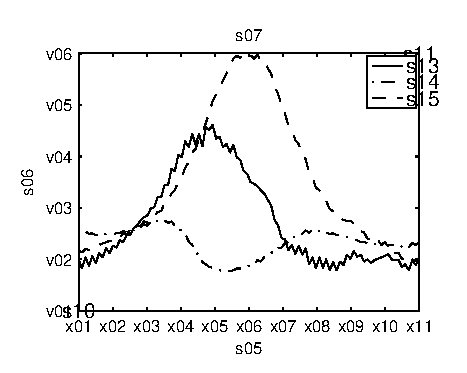
\includegraphics{est_data_one.eps}}%
% \end{psfrags}%
% %
% End est_data_one.tex

    \includegraphics[width=\linewidth]{images/meas_data_one}
   \caption[Data from estimated parameters, one magnetic moment.]{Data from estimated parameters. One magnetic moment was estimated.}
   \label{fig-est_data_one}
   \end{minipage}
  \end{figure}
\end{subfigures}

\section{Verification of algorithms}

Measurements done with our prototype node can be seen in Figure~\ref{fig-traffic}. The frequency content can be seen in Figure~\ref{fig-traffic_fft}. The signal contains a lot of power around 50~Hz which is expected. Noteworthy is that the signal contains most of its power at very low frequencies, and therefore we can use a crude filter to get rid of the noise at higher frequencies. The influence of the 50~Hz frequencies was later made smaller by the use of a 2nd order IIR notch filter. We can see that the vehicle signatures are much higher in amplitude than the noise. The large signature in the data in Figure~\ref{fig-traffic} comes from a large double-deck bus.

\begin{subfigures}
\begin{figure}[!htb]
  \centering
  \begin{minipage}{0.45\linewidth}
  \centering
   % generated by laprint.m
%
% \begin{psfrags}%
% \psfragscanon%
%
% text strings:
\psfrag{s02}[b][b]{\fontsize{8}{12}\fontseries{m}\mathversion{normal}\fontshape{n}\selectfont \setlength{\tabcolsep}{0pt}\begin{tabular}{c}Traffic Sequence (filtered data)\end{tabular}}%
\psfrag{s03}[t][t]{\fontsize{8}{12}\fontseries{m}\mathversion{normal}\fontshape{n}\selectfont \setlength{\tabcolsep}{0pt}\begin{tabular}{c}Samples\end{tabular}}%
\psfrag{s04}[b][b]{\fontsize{8}{12}\fontseries{m}\mathversion{normal}\fontshape{n}\selectfont \setlength{\tabcolsep}{0pt}\begin{tabular}{c}Magnetic field strength [nT]\end{tabular}}%
%
% axes font properties:
\fontsize{6}{8}\fontseries{m}\mathversion{normal}%
\fontshape{n}\selectfont%
%
% xticklabels:
\psfrag{x01}[t][t]{$0$}%
\psfrag{x02}[t][t]{$0.5$}%
\psfrag{x03}[t][t]{$1$}%
\psfrag{x04}[t][t]{$1.5$}%
\psfrag{x05}[t][t]{$2$}%
\psfrag{x06}[t][t]{$2.5$}%
\psfrag{x07}[t][t]{$3$}%
%
% yticklabels:
\psfrag{v01}[r][r]{$-8000$}%
\psfrag{v02}[r][r]{$-6000$}%
\psfrag{v03}[r][r]{$-4000$}%
\psfrag{v04}[r][r]{$-2000$}%
\psfrag{v05}[r][r]{$0$}%
\psfrag{v06}[r][r]{$2000$}%
\psfrag{v07}[r][r]{$4000$}%
\psfrag{v08}[r][r]{$6000$}%
\psfrag{v09}[r][r]{$8000$}%
%
% Figure:
% \resizebox{6cm}{!}{\includegraphics{traffic_data_filt.eps}}%
% \end{psfrags}%
%
% End traffic_data_filt.tex

   \includegraphics[width=\linewidth]{images/traffic_data_filt}
  \caption[Measured data from traffic.]{Measured data from traffic. The signal was filtered using a low order digital lowpass filter.}
  \label{fig-traffic}
  \end{minipage}\hfill
  \begin{minipage}{0.45\linewidth}
   \centering
     % generated by laprint.m
% %
% \begin{psfrags}%
% \psfragscanon%
% %
% text strings:
\psfrag{s02}[t][t]{\fontsize{8}{12}\fontseries{m}\mathversion{normal}\fontshape{n}\selectfont \setlength{\tabcolsep}{0pt}\begin{tabular}{c}Frequency [Hz]\end{tabular}}%
\psfrag{s03}[b][b]{\fontsize{8}{12}\fontseries{m}\mathversion{normal}\fontshape{n}\selectfont \setlength{\tabcolsep}{0pt}\begin{tabular}{c}$\vert{}Y(f)\vert$\end{tabular}}%
\psfrag{s04}[b][b]{\fontsize{8}{12}\fontseries{m}\mathversion{normal}\fontshape{n}\selectfont \setlength{\tabcolsep}{0pt}\begin{tabular}{c}FFT of unfiltered data\end{tabular}}%
%
% axes font properties:
\fontsize{6}{8}\fontseries{m}\mathversion{normal}%
\fontshape{n}\selectfont%
%
% xticklabels:
\psfrag{x01}[t][t]{$0$}%
\psfrag{x02}[t][t]{$5$}%
\psfrag{x03}[t][t]{$10$}%
\psfrag{x04}[t][t]{$15$}%
\psfrag{x05}[t][t]{$20$}%
\psfrag{x06}[t][t]{$25$}%
\psfrag{x07}[t][t]{$30$}%
\psfrag{x08}[t][t]{$35$}%
\psfrag{x09}[t][t]{$40$}%
\psfrag{x10}[t][t]{$45$}%
\psfrag{x11}[t][t]{$50$}%
%
% yticklabels:
\psfrag{v01}[r][r]{$0$}%
\psfrag{v02}[r][r]{$0.05$}%
\psfrag{v03}[r][r]{$0.1$}%
\psfrag{v04}[r][r]{$0.15$}%
\psfrag{v05}[r][r]{$0.2$}%
\psfrag{v06}[r][r]{$0.25$}%
\psfrag{v07}[r][r]{$0.3$}%
\psfrag{v08}[r][r]{$0.35$}%
\psfrag{v09}[r][r]{$0.4$}%
%
% % Figure:
% \resizebox{6cm}{!}{\includegraphics{traffic_data_fft.eps}}%
% \end{psfrags}%
% %
% End traffic_data_fft.tex

   \includegraphics[width=\linewidth]{images/traffic_data_fft}
  \caption[FFT of measured data from traffic.]{FFT of measured data from traffic. Unfiltered data.}
  \label{fig-traffic_fft}
  \end{minipage}
 \end{figure}
\end{subfigures}

It is worth noting that if we have traffic travelling in the other direction, we can eliminate them using their speed estimation. Of 18 vehicles travelling in the positive direction, 18 are detected. This is of course a very short sample, and more measurements have to be done. If a driver is instructed to pass the sensors at 50~km/h, the result differs from that velocity by a maximum of 2~km/h when the matched filter method was used. The number of vehicle passings was only thirteen. Due to the limited use of the experiment data, a velocity control measurement was deemed necessary.

The most energy in the signal can be found at low frequencies which means that we can use a low pass filter to get rid of undesired high frequency content.

\begin{subfigures}
\begin{figure}[!ht]
  \centering
  	\begin{minipage}{0.45\linewidth}
  \centering
  % generated by laprint.m
%
% \begin{psfrags}%
% \psfragscanon%
% %
% text strings:
\psfrag{s05}[t][t]{\fontsize{8}{12}\fontseries{m}\mathversion{normal}\fontshape{n}\selectfont \setlength{\tabcolsep}{0pt}\begin{tabular}{c}Samples\end{tabular}}%
\psfrag{s06}[b][b]{\fontsize{8}{12}\fontseries{m}\mathversion{normal}\fontshape{n}\selectfont \setlength{\tabcolsep}{0pt}\begin{tabular}{c}Magnetic field strength [uT]\end{tabular}}%
\psfrag{s08}[b][b]{\fontsize{8}{12}\fontseries{m}\mathversion{normal}\fontshape{n}\selectfont \setlength{\tabcolsep}{0pt}\begin{tabular}{c}Vehicle detection\end{tabular}}%
\psfrag{s10}[][]{\fontsize{8}{12}\fontseries{m}\mathversion{normal}\fontshape{n}\selectfont \setlength{\tabcolsep}{0pt}\begin{tabular}{c} \end{tabular}}%
\psfrag{s11}[][]{\fontsize{8}{12}\fontseries{m}\mathversion{normal}\fontshape{n}\selectfont \setlength{\tabcolsep}{0pt}\begin{tabular}{c} \end{tabular}}%
\psfrag{s12}[l][l]{\fontsize{6}{8}\fontseries{m}\mathversion{normal}\fontshape{n}\selectfont 2nd node}%
\psfrag{s13}[l][l]{\fontsize{6}{8}\fontseries{m}\mathversion{normal}\fontshape{n}\selectfont 1st node}%
\psfrag{s14}[l][l]{\fontsize{6}{8}\fontseries{m}\mathversion{normal}\fontshape{n}\selectfont 2nd node}%
%
% axes font properties:
\fontsize{6}{8}\fontseries{m}\mathversion{normal}%
\fontshape{n}\selectfont%
%
% xticklabels:
\psfrag{x01}[t][t]{$0$}%
\psfrag{x02}[t][t]{$20$}%
\psfrag{x03}[t][t]{$40$}%
\psfrag{x04}[t][t]{$60$}%
\psfrag{x05}[t][t]{$80$}%
\psfrag{x06}[t][t]{$100$}%
\psfrag{x07}[t][t]{$120$}%
\psfrag{x08}[t][t]{$140$}%
\psfrag{x09}[t][t]{$160$}%
\psfrag{x10}[t][t]{$180$}%
\psfrag{x11}[t][t]{$200$}%
%
% yticklabels:
\psfrag{v01}[r][r]{$-6$}%
\psfrag{v02}[r][r]{$-4$}%
\psfrag{v03}[r][r]{$-2$}%
\psfrag{v04}[r][r]{$0$}%
\psfrag{v05}[r][r]{$2$}%
\psfrag{v06}[r][r]{$4$}%
\psfrag{v07}[r][r]{$6$}%
\psfrag{v08}[r][r]{$8$}%
\psfrag{v09}[r][r]{$10$}%
\psfrag{v10}[r][r]{$12$}%
%
% Figure:
% \resizebox{6cm}{!}{\includegraphics{vehicledet.eps}}%
% \end{psfrags}%
%
% End vehicledet.tex

   \includegraphics[width=\linewidth]{images/vehicledet}
  \caption[Two-node vehicle detection]{Two-node vehicle detection. The distance between the curves determine the speed of the vehicle.}
  \label{fig:vehicledet}
  \end{minipage}\hfill
  \begin{minipage}{0.45\linewidth}
   \centering
   % generated by laprint.m
%
% \begin{psfrags}%
% \psfragscanon%
%
% text strings:
\psfrag{s02}[b][b]{\fontsize{8}{12}\fontseries{m}\mathversion{normal}\fontshape{n}\selectfont \setlength{\tabcolsep}{0pt}\begin{tabular}{c}Convolution\end{tabular}}%
\psfrag{s03}[b][b]{\fontsize{8}{12}\fontseries{m}\mathversion{normal}\fontshape{n}\selectfont \setlength{\tabcolsep}{0pt}\begin{tabular}{c}f*g\end{tabular}}%
\psfrag{s04}[t][t]{\fontsize{8}{12}\fontseries{m}\mathversion{normal}\fontshape{n}\selectfont \setlength{\tabcolsep}{0pt}\begin{tabular}{c}Samples\end{tabular}}%
%
% axes font properties:
\fontsize{6}{8}\fontseries{m}\mathversion{normal}%
\fontshape{n}\selectfont%
%
% xticklabels:
\psfrag{x01}[t][t]{$0$}%
\psfrag{x02}[t][t]{$50$}%
\psfrag{x03}[t][t]{$100$}%
\psfrag{x04}[t][t]{$150$}%
\psfrag{x05}[t][t]{$200$}%
\psfrag{x06}[t][t]{$250$}%
\psfrag{x07}[t][t]{$300$}%
\psfrag{x08}[t][t]{$350$}%
\psfrag{x09}[t][t]{$400$}%
%
% yticklabels:
\psfrag{v01}[r][r]{$-1000$}%
\psfrag{v02}[r][r]{$-500$}%
\psfrag{v03}[r][r]{$0$}%
\psfrag{v04}[r][r]{$500$}%
\psfrag{v05}[r][r]{$1000$}%
\psfrag{v06}[r][r]{$1500$}%
\psfrag{v07}[r][r]{$2000$}%
\psfrag{v08}[r][r]{$2500$}%
%
% Figure:
% \resizebox{6cm}{!}{\includegraphics{conv.eps}}%
% \end{psfrags}%
%
% End conv.tex

   \includegraphics[width=\linewidth]{images/conv}
  \caption[Matched filter method. Convolution result.]{Convolution of the first and second node data. The peak is clearly visible.\\}
  \label{fig:conv}
  \end{minipage}
 \end{figure}
 \end{subfigures}

 The result of the convolution of the two sensor node outputs seen in Figure~\ref{fig:vehicledet} can be seen in Figure~\ref{fig:conv}. We can see that the peak is well defined, and not noisy. In fact, the sensor node signals can be much more noisy as described earlier. An example of an interpolation around the peak can be seen in Figure~\ref{fig:reconst}.

%  \begin{subfigures}
\begin{figure}[!ht]
  \centering
  	\begin{minipage}{0.45\linewidth}
  \centering
  % generated by laprint.m
%
% \begin{psfrags}%
% \psfragscanon%
%
% text strings:
\psfrag{s02}[b][b]{\fontsize{8}{12}\fontseries{m}\mathversion{normal}\fontshape{n}\selectfont \setlength{\tabcolsep}{0pt}\begin{tabular}{c}Sinc reconstruction\end{tabular}}%
\psfrag{s03}[t][t]{\fontsize{8}{12}\fontseries{m}\mathversion{normal}\fontshape{n}\selectfont \setlength{\tabcolsep}{0pt}\begin{tabular}{c}Time [s]\end{tabular}}%
\psfrag{s04}[b][b]{\fontsize{8}{12}\fontseries{m}\mathversion{normal}\fontshape{n}\selectfont \setlength{\tabcolsep}{0pt}\begin{tabular}{c}Correlation\end{tabular}}%
%
% axes font properties:
\fontsize{6}{8}\fontseries{m}\mathversion{normal}%
\fontshape{n}\selectfont%
%
% xticklabels:
\psfrag{x01}[t][t]{$218$}%
\psfrag{x02}[t][t]{$220$}%
\psfrag{x03}[t][t]{$222$}%
\psfrag{x04}[t][t]{$224$}%
\psfrag{x05}[t][t]{$226$}%
\psfrag{x06}[t][t]{$228$}%
%
% yticklabels:
\psfrag{v01}[r][r]{$-40$}%
\psfrag{v02}[r][r]{$-20$}%
\psfrag{v03}[r][r]{$0$}%
\psfrag{v04}[r][r]{$20$}%
\psfrag{v05}[r][r]{$40$}%
\psfrag{v06}[r][r]{$60$}%
\psfrag{v07}[r][r]{$80$}%
\psfrag{v08}[r][r]{$100$}%
\psfrag{v09}[r][r]{$120$}%
%
% % Figure:
% \resizebox{6cm}{!}{\includegraphics{reconst.eps}}%
% \end{psfrags}%
%
% End reconst.tex

   \includegraphics[width=\linewidth]{images/reconst}
  \caption[Sinc reconstruction]{Sinc reconstruction of the convolution peak.}
  \label{fig:reconst}
  \end{minipage}
% \hfill
%   \begin{minipage}{0.45\linewidth}
%    \centering
%    % generated by laprint.m
%
% \begin{psfrags}%
% \psfragscanon%
%
% text strings:
\psfrag{s02}[b][b]{\fontsize{8}{12}\fontseries{m}\mathversion{normal}\fontshape{n}\selectfont \setlength{\tabcolsep}{0pt}\begin{tabular}{c}Sinc reconstruction\end{tabular}}%
\psfrag{s03}[t][t]{\fontsize{8}{12}\fontseries{m}\mathversion{normal}\fontshape{n}\selectfont \setlength{\tabcolsep}{0pt}\begin{tabular}{c}Time [s]\end{tabular}}%
\psfrag{s04}[b][b]{\fontsize{8}{12}\fontseries{m}\mathversion{normal}\fontshape{n}\selectfont \setlength{\tabcolsep}{0pt}\begin{tabular}{c}Correlation\end{tabular}}%
%
% axes font properties:
\fontsize{6}{8}\fontseries{m}\mathversion{normal}%
\fontshape{n}\selectfont%
%
% xticklabels:
\psfrag{x01}[t][t]{$222.2$}%
\psfrag{x02}[t][t]{$222.4$}%
\psfrag{x03}[t][t]{$222.6$}%
\psfrag{x04}[t][t]{$222.8$}%
\psfrag{x05}[t][t]{$223$}%
\psfrag{x06}[t][t]{$223.2$}%
\psfrag{x07}[t][t]{$223.4$}%
\psfrag{x08}[t][t]{$223.6$}%
\psfrag{x09}[t][t]{$223.8$}%
%
% yticklabels:
\psfrag{v01}[r][r]{$103.4$}%
\psfrag{v02}[r][r]{$103.6$}%
\psfrag{v03}[r][r]{$103.8$}%
\psfrag{v04}[r][r]{$104$}%
\psfrag{v05}[r][r]{$104.2$}%
\psfrag{v06}[r][r]{$104.4$}%
\psfrag{v07}[r][r]{$104.6$}%
\psfrag{v08}[r][r]{$104.8$}%
\psfrag{v09}[r][r]{$105$}%
\psfrag{v10}[r][r]{$105.2$}%
%
% % Figure:
% \resizebox{6cm}{!}{\includegraphics{reconstzoom.eps}}%
% \end{psfrags}%
%
% End reconstzoom.tex

%    \includegraphics[width=\linewidth]{images/reconstzoom}
%   \caption[Matched filter method. Convolution result.]{Convolution of the first and second node data. The peak is clearly visible.\\}
%   \label{fig:reconstzoom}
%   \end{minipage}
 \end{figure}
%  \end{subfigures}

 In the result we can see that the estimated speeds do not differ by much when we use different sensor axis. We also note that the difference in sensor sensitivity does contribute in the sense that we have to use a different threshold but not otherwise. This is a huge improvement over the peak to peak method used in other publications.

